%
% Template Laporan Skripsi/Thesis 
%
% @author  Andreas Febrian, Lia Sadita 
% @version 1.03
%
% Dokumen ini dibuat berdasarkan standar IEEE dalam membuat class untuk 
% LaTeX dan konfigurasi LaTeX yang digunakan Fahrurrozi Rahman ketika 
% membuat laporan skripsi. Konfigurasi yang lama telah disesuaikan dengan 
% aturan penulisan thesis yang dikeluarkan UI pada tahun 2008.
%

%
% Tipe dokumen adalah report dengan satu kolom. 
%
\documentclass[12pt, a4paper, onecolumn, oneside, final]{report}

% Load konfigurasi LaTeX untuk tipe laporan thesis
\usepackage{tikz}
\usetikzlibrary{shapes.geometric, arrows, positioning, fit, calc} % Untuk diagram alur
\usepackage{_internals/uithesis}
\usepackage{alltt}
\usepackage{amsmath}
\usepackage{pgfplots}
\usepackage{listings}
\usepackage{multicol}
\usepackage{pdfpages}
\usepackage{xcolor}
\usepackage{booktabs}
\usepackage{tabularx}
\usepackage{pgfplots}

\pgfplotsset{compat=1.18}
\lstset{breaklines=true} 

% Daftar pemenggalan suku kata dan istilah dalam LaTeX
%
% Hyphenation untuk Indonesia 
%
% @author  Andreas Febrian
% @version 1.00
% 
% Tambahkan cara pemenggalan kata-kata yang salah dipenggal secara otomatis 
% oleh LaTeX. Jika kata tersebut dapat dipenggal dengan benar, maka tidak 
% perlu ditambahkan dalam berkas ini. Tanda pemenggalan kata menggunakan 
% tanda '-'; contoh:
% menarik
%   --> pemenggalan: me-na-rik
%

\hyphenation{
    % alphabhet A
    a-na-li-sa a-tur 
    a-pli-ka-si 
    % alphabhet B
    ba-ngun-an 
    be-be-ra-pa 
    ber-ge-rak
    ber-ke-lan-jut-an 
    ber-pe-nga-ruh 
    % alphabhet C
    ca-ri
    % alphabhet D
    di-sim-pan di-pim-pin de-ngan da-e-rah di-ba-ngun da-pat di-nya-ta-kan 
    di-sim-bol-kan di-pi-lih di-li-hat de-fi-ni-si
    % alphabhet E
    e-ner-gi eks-klu-sif
    % alphabhet F
    fa-si-li-tas
    % alphabhet G
    ga-bung-an ge-rak
    % alphabhet H
    ha-lang-an
    % alphabhet I
    % alphabhet J
    % alphabhet K
    ke-hi-lang-an
    ku-ning 
    kua-li-tas ka-me-ra ke-mung-kin-an ke-se-pa-ham-an
    % alphabhet L
    ling-kung-an
    % alphabhet M
    me-neng-ah
    meng-a-tas-i me-mung-kin-kan me-nge-na-i me-ngi-rim-kan 
    meng-u-bah meng-a-dap-ta-si me-nya-ta-kan mo-di-fi-ka-si
    meng-a-tur
    % alphabhet N
    nya-ta non-eks-klu-sif
    % alphabhet O
    % alphabhet P
	pe-nye-rap-an 
	pe-ngon-trol
    pe-mo-del-an
    pe-ran  pe-ran-an-nya
    pem-ba-ngun-an pre-si-den pe-me-rin-tah prio-ri-tas peng-am-bil-an 
    peng-ga-bung-an pe-nga-was-an pe-ngem-bang-an 
    pe-nga-ruh pa-ra-lel-is-me per-hi-tung-an per-ma-sa-lah-an 
    pen-ca-ri-an peng-struk-tur-an
    % alphabhet Q
    % alphabhet R
    ran-cang-an
    % alphabhet S
    si-mu-la-si sa-ngat
    % alphabhet T
    te-ngah
    ter-da-pat
    % alphabhet U
    % alphabhet V
    % alphabhet W
    % alphabhet X
    % alphabhet Y
    % alphabhet Z
    % special
}

% Load konfigurasi khusus untuk laporan yang sedang dibuat
%-----------------------------------------------------------------------------%
% Informasi Mengenai Dokumen
%-----------------------------------------------------------------------------%
% 
% Judul laporan. 
\var{\judul}{Implementasi dan Analisis Efektivitas \f{Code Virtualization} dalam Meningkatkan Keamanan \f{Software} dengan Mempersulit \f{Reverse Engineering} menggunakan VxLang}
% 
% Tulis kembali judul laporan, kali ini akan diubah menjadi huruf kapital
\Var{\Judul}{Implementasi dan Analisis Efektivitas \f{Code Virtualization} dalam Meningkatkan Keamanan \f{Software} dengan Mempersulit \f{Reverse Engineering} menggunakan VxLang}
% 
% Tulis kembali judul laporan namun dengan bahasa Ingris
\var{\judulInggris}{Implementation and Analysis of the Effectiveness of Code Virtualization in Improving Software Security by complicating Reverse Engineering}
% 
% Tipe laporan, dapat berisi Skripsi, Tugas Akhir, Thesis, atau Disertasi
\var{\type}{Skripsi}
% 
% Tulis kembali tipe laporan, kali ini akan diubah menjadi huruf kapital
\Var{\Type}{Skripsi}
% 
% Tulis nama penulis 
\var{\penulis}{Seno Pamungkas Rahman}
% 
% Tulis kembali nama penulis, kali ini akan diubah menjadi huruf kapital
\Var{\Penulis}{Seno Pamungkass Rahman}
% 
% Tulis NPM penulis
\var{\npm}{2106731586}
% 
% Tuliskan Fakultas dimana penulis berada
\Var{\Fakultas}{Teknik}
\var{\fakultas}{Teknik}
% 
% Tuliskan Program Studi yang diambil penulis
\Var{\Program}{Teknik Komputer}
\var{\program}{Teknik Komputer}
% 
% Tuliskan tahun publikasi laporan
\Var{\bulan}{Januari}
\Var{\tahun}{2025}
% 
% Tuliskan gelar yang akan diperoleh dengan menyerahkan laporan ini
\var{\gelar}{Sarjana Teknik}
% 
% Tuliskan tanggal pengesahan laporan, waktu dimana laporan diserahkan ke 
% penguji/sekretariat
\var{\tanggalPengesahan}{Januari 2025}
% 
% Tuliskan tanggal keputusan sidang dikeluarkan dan penulis dinyatakan 
% lulus/tidak lulus
\var{\tanggalLulus}{Januari 2025}
% 
% Tuliskan pembimbing 
\var{\pembimbing}{Dr. Ruki Harwahyu, S.T. M.T. MSc.}
% 
% Tuliskan penguji
\var{\pengujisatu}{Dr. Ruki Harwahyu, ST. MT. MSc.}
\var{\pengujidua}{I Gde Dharma Nugraha, S.T., M.T., Ph.D}
% 
% Alias untuk memudahkan alur penulisan paa saat menulis laporan
\var{\saya}{Penulis}

%-----------------------------------------------------------------------------%
% Judul Setiap Bab
%-----------------------------------------------------------------------------%
% 
% Berikut ada judul-judul setiap bab. 
% Silahkan diubah sesuai dengan kebutuhan. 
% 
\Var{\kataPengantar}{Kata Pengantar}
\Var{\babSatu}{Pendahuluan}
\Var{\babDua}{Tinjauan Pustaka}
\Var{\babTiga}{Metode Penelitian}
\Var{\babEmpat}{Implementasi}
\Var{\babLima}{Hasil Penelitian}
\Var{\babEnam}{Kesimpulan dan Saran}

% Daftar istilah yang mungkin perlu ditandai 
%
% @author  Andreas Febrian
% @version 1.00
% 
% Mendaftar seluruh istilah yang mungkin akan perlu dijadikan 
% italic atau bold pada setiap kemunculannya dalam dokumen. 
% 

\var{\license}{\f{Creative Common License 1.0 Generic}}
\var{\bslash}{$\setminus$}

%\var{\cc}{\f{Cloud Computing}}
%\var{\vm}{\f{Virtual Machine}}
%\var{\vmm}{\f{Virtual Machine Monitor}}
%\var{\oss}{\f{open source}}
%\var{\ssim}{\f{Structural Similarity Index Measure}}


% Awal bagian penulisan laporan
\begin{document}
%
% Sampul Laporan
%
% Sampul Laporan

%
% @author  unknown
% @version 1.01
% @edit by Andreas Febrian
%

\begin{titlepage}
    \begin{center}    
        \begin{figure}
            \begin{center}
                
\includegraphics[width=2.5cm]{assets/pics/makara_yellow.png}
            \end{center}
        \end{figure}    
        \vspace*{0cm}
        \bo{
        	UNIVERSITAS INDONESIA\\
        }
        
        \vspace*{1.0cm}
        % judul thesis harus dalam 14pt Times New Roman
        \bo{\Judul} \\[1.0cm]

        \vspace*{2.5 cm}    
        % harus dalam 14pt Times New Roman
        \bo{\Type}

        \vspace*{3 cm}       
        % penulis dan npm
        \bo{\Penulis} \\
        \bo{\npm} \\

        \vspace*{5.0cm}

        % informasi mengenai fakultas dan program studi
        \bo{
        	FAKULTAS \Fakultas\\
        	PROGRAM STUDI \Program \\
        	DEPOK \\
        	\tahun
        }
    \end{center}
\end{titlepage}


%
% Gunakan penomeran romawi
\pagenumbering{roman}

%
% load halaman judul dalam
\addChapter{HALAMAN JUDUL}
%
% Halaman Judul Laporan 
%
% @author  unknown
% @version 1.01
% @edit by Andreas Febrian
%


\begin{titlepage}
    \begin{center}\begin{figure}
            \begin{center}
                
\includegraphics[width=2.5cm]{_internals/makara.eps}
            \end{center}
        \end{figure}    
        \vspace*{0cm}
        \bo{
        	UNIVERSITAS INDONESIA\\
        }
        
        \vspace*{1.0cm}
        % judul thesis harus dalam 14pt Times New Roman
        \bo{\Judul} \\[1.0cm]

        \vspace*{2.5 cm}    
        % harus dalam 14pt Times New Roman
        \bo{\Type} \\
        % keterangan prasyarat
        \bo{Diajukan sebagai salah satu syarat untuk memperoleh gelar \\
        \gelar}\\

        \vspace*{3 cm}       
        % penulis dan npm
        \bo{\Penulis} \\
        \bo{\npm} \\

        \vspace*{4.0cm}

        % informasi mengenai fakultas dan program studi
        \bo{
        	FAKULTAS \Fakultas\\
        	PROGRAM STUDI \Program \\
        	DEPOK \\
        	\bulan\ \tahun
        }
    \end{center}
\end{titlepage}

%
% setelah bagian ini, halaman dihitung sebagai halaman ke 2
\setcounter{page}{2}

%
% load halaman pengesahan
%\addChapter{LEMBAR PERSETUJUAN}
%%
% Halaman Pengesahan
%
% @author  Andreas Febrian
% @version 1.01
%

\chapter*{HALAMAN PERSETUJUAN}

\vspace*{0.2cm}
\noindent

\noindent
\begin{tabular}{l l p{11cm}}
	\bo{Judul} & : & \judul   \\
	\bo{Penulis}  & : & \penulis \\
	\bo{NPM}   & : & \npm     \\
\end{tabular} \\

\vspace*{1.2cm}

\noindent Laporan \type~ini telah diperiksa dan disetujui.\\[0.3cm]
\begin{center}
	\tanggalPengesahan \\[2cm]


	\underline{\pembimbing}\\[0.1cm]
	Pembimbing \type
\end{center}

\newpage

%
% load halaman orisinalitas 
\addChapter{LEMBAR PERNYATAAN ORISINALITAS}
%
% Halaman Orisinalitas
%
% @author  Andreas Febrian
% @version 1.01
%

\chapter*{Halaman Pernyataan Orisinalitas}
\vspace*{2cm}

\begin{center}
	\bo{\type~ini adalah hasil karya saya sendiri, \\
		dan semua sumber baik yang dikutip maupun dirujuk \\
		telah saya nyatakan dengan benar.} \\
	\vspace*{2.6cm}

	\begin{tabular}{l c l}
		\bo{Nama}         & : & \bo{\penulis}           \\
		\bo{NPM}          & : & \bo{\npm}               \\
		\bo{Tanda Tangan} & : &                         \\
		                  &   &                         \\
		                  &   &                         \\
		\bo{Tanggal}      & : & \bo{\tanggalPengesahan} \\
	\end{tabular}
\end{center}

\newpage
%
%
\addChapter{LEMBAR PENGESAHAN}
%
% Halaman Pengesahan Sidang
%
% @author  Andreas Febrian, Andre Tampubolon 
% @version 1.02
%

\chapter*{HALAMAN PENGESAHAN}

\vspace*{0.4cm}
\noindent

\noindent
\begin{tabular}{ll p{9cm}}
	\type~ini diajukan oleh & : &          \\
	Nama                    & : & \penulis \\
	NPM                     & : & \npm     \\
	Program Studi           & : & \program \\
	Judul \type             & : & \judul   \\
\end{tabular} \\

\vspace*{1.0cm}

\noindent \bo{Telah berhasil dipertahankan di hadapan Dewan Penguji
	dan diterima sebagai bagian persyaratan yang diperlukan untuk
	memperoleh gelar \gelar~pada Program Studi \program, Fakultas
	\fakultas, Universitas Indonesia.}\\[0.2cm]

\begin{center}
	\bo{DEWAN PENGUJI}
\end{center}

\vspace*{0.3cm}

\begin{tabular}{l l l l }
	           &   &              &                   \\
	Pembimbing & : & \pembimbing  & (\hspace*{3.0cm}) \\
	           &   &              &                   \\
	Penguji    & : & \pengujisatu & (\hspace*{3.0cm}) \\
	           &   &              &                   \\
	Penguji    & : & \pengujidua  & (\hspace*{3.0cm}) \\
\end{tabular}\\

%\todo{Jangan lupa mengisi nama para penguji.}

\vspace*{2.0cm}

\begin{tabular}{ll l}
	Ditetapkan di & : & Depok         \\
	Tanggal       & : & \tanggalLulus \\
\end{tabular}


\newpage
%
%
\addChapter{\kataPengantar}
%-----------------------------------------------------------------------------%
\chapter*{Kata Pengantar}
%-----------------------------------------------------------------------------%
Penulis mengucapkan terima kasih kepada :

    1. Dr. Ruki Harwahyu, ST, MT, MSc. dosen pembimbing atas segala bimbingan, ilmu, dan arahan baik dalam penulisan skripsi maupun selama masa studi di Teknik Komputer.
    2. Orang tua dan keluarga yang telah memberikan bantuan dukungan material dan moral.
    3. Teman-teman di program studi Teknik Koputer atas segala dukungan dan kerja samanya.

sehingga penulisan skripsi ini dapat diselesaikan dengan baik dan benar. Akhir kata, penulis  berharap Tuhan Yang Maha Esa berkenan membalas segala kebaikan semua pihak yang telah membantu. Penulis berharap kritik dan saran untuk melengkapi kekurangan pada skripsi ini.


\vspace*{0.1cm}
\begin{flushright}
	Depok, 3 Januari 2025\\[0.1cm]
	\vspace*{1cm}
	\penulis

\end{flushright}

%
%
\addChapter{LEMBAR PERSETUJUAN PUBLIKASI ILMIAH}
% 
% @author  Andre Tampubolon, Andreas Febrian
% @version 1.01
% 

\chapter*{Halaman Pernyataan Persetujuan Publikasi Tugas Akhir untuk Kepentingan Akademis}

\vspace*{0.2cm}
\noindent
Sebagai sivitas akademik Universitas Indonesia, saya yang bertanda
tangan di bawah ini:
\vspace*{0.4cm}


\begin{tabular}{p{4.2cm} l p{6cm}}
	\bo{Nama}          & : & \penulis  \\
	\bo{NPM}           & : & \npm      \\
	\bo{Program Studi} & : & \program  \\
	\bo{Fakultas}      & : & \fakultas \\
	\bo{Jenis Karya}   & : & \type     \\
\end{tabular}

\vspace*{0.6cm}
\noindent demi pengembangan ilmu pengetahuan, menyetujui untuk memberikan
kepada Universitas Indonesia \bo{Hak Bebas Royalti Noneksklusif
	(\textit{Non-exclusive Royalty Free Right})} atas karya ilmiah saya yang berjudul:
\begin{center}
	\judul
\end{center}
beserta perangkat yang ada (jika diperlukan). Dengan Hak Bebas Royalti
Noneksklusif ini Universitas Indonesia berhak menyimpan,
mengalihmedia/formatkan, mengelola dalam bentuk pangkalan data
(\textit{database}), merawat, dan memublikasikan tugas akhir saya selama
tetap mencantumkan nama saya sebagai penulis/pencipta dan sebagai
pemilik Hak Cipta. \\

\noindent Demikian pernyatan ini saya buat dengan sebenarnya.

\begin{center}
	\vspace*{0.8cm}
	\begin{tabular}{rl}
		Dibuat di :    & Depok              \\
		Pada tanggal : & \tanggalPengesahan \\
	\end{tabular}\\

	\vspace*{0.2cm}
	Yang menyatakan \\
	\vspace*{1.1cm}
	(\penulis)
\end{center}

\newpage


%
% 
\addChapter{ABSTRAK}
%
% Halaman Abstrak
%
% @author  Andreas Febrian
% @version 1.00
%

\chapter*{Abstrak}

\vspace*{0.2cm}
{
	\setlength{\parindent}{0pt}

	\begin{tabular}{@{}l l p{10cm}}
		Nama          & : & \penulis    \\
		Program Studi & : & \program    \\
		Judul         & : & \judul      \\
		Pembimbing    & : & \pembimbing \\
	\end{tabular}

	\bigskip
	\bigskip

	\cc\ Rekayasa balik merupakan ancaman serius terhadap keamanan perangkat lunak, memungkinkan penyerang untuk menganalisis, memahami, dan memodifikasi kode program tanpa izin. Teknik obfuscation, terutama virtualisasi kode, menjadi solusi yang menjanjikan untuk melindungi perangkat lunak dari ancaman ini. Penelitian ini bertujuan untuk mengimplementasikan dan menganalisis efektivitas virtualisasi kode dalam meningkatkan keamanan perangkat lunak dengan mempersulit rekayasa balik. Penelitian ini menggunakan EagleVM sebagai platform virtualisasi kode. Metode penelitian yang digunakan meliputi implementasi virtualisasi kode pada sebuah aplikasi studi kasus, kemudian dilakukan analisis statis dan dinamis terhadap aplikasi sebelum dan sesudah di-obfuscate. Analisis statis dilakukan dengan membandingkan tingkat kesulitan dalam memahami kode assembly yang dihasilkan. Analisis dinamis dilakukan dengan mengukur waktu eksekusi dan sumber daya yang digunakan oleh aplikasi. Hasil penelitian menunjukkan bahwa virtualisasi kode dengan EagleVM efektif dalam meningkatkan keamanan perangkat lunak. Kode yang telah di-obfuscate menjadi lebih sulit dipahami dan dianalisis, terlihat dari meningkatnya kompleksitas kode assembly. Penelitian ini diharapkan dapat membuktikan bahwa virtualisasi kode dengan EagleVM merupakan teknik yang efektif untuk melindungi perangkat lunak dari rekayasa balik dan dapat dipertimbangkan sebagai solusi untuk meningkatkan keamanan aplikasi.

	\bigskip

	Kata kunci:\\
	Pengaburan Kode, Virtualisasi Kode, Perlindungan Perangkat Lunak, Rekayasa Balik
}

\newpage

%
%
%
% Halaman Abstract
%
% @author  Andreas Febrian
% @version 1.00
%

\chapter*{Abstract}

\vspace*{0.2cm}
{
	\setlength{\parindent}{0pt}

	\begin{tabular}{@{}l l p{10cm}}
		Name          & : & \penulis      \\
		Study Program & : & \program      \\
		Title         & : & \judulInggris \\
		Counsellor    & : & \pembimbing   \\
	\end{tabular}

	\bigskip
	\bigskip

Reverse engineering is a serious threat to software security, allowing attackers to analyze, understand, and modify program code without permission. Obfuscation techniques, especially code virtualization, are promising solutions to protect software from this threat. This study aims to implement and analyze the effectiveness of code virtualization in improving software security by complicating reverse engineering. This study uses EagleVM as a code virtualization platform. The research methods used include implementing code virtualization on a case study application, then conducting static and dynamic analysis of the application before and after obfuscation. Static analysis is done by comparing the level of difficulty in understanding the resulting assembly code. Dynamic analysis is done by measuring the execution time and resources used by the application. The results of the study show that code virtualization with EagleVM is effective in improving software security. Obfuscated code becomes more difficult to understand and analyze, as seen from the increasing complexity of the assembly code. This study is expected to prove that code virtualization with EagleVM is an effective technique to protect software from reverse engineering and can be considered as a solution to improve application security.

	\bigskip

	Key words:\\
	Code Obfuscation, Code Virtualization, Software Protection, Reverse Engineering
}

\newpage


%
% Daftar isi, gambar, dan tabel
%
\phantomsection
\tableofcontents
\clearpage
\phantomsection
\listoffigures
\clearpage
\phantomsection
\listoftables
\clearpage
\phantomsection
\addcontentsline{toc}{chapter}{\uppercase{Daftar Kode}}
\listoflistings
\clearpage

%
% Gunakan penomeran Arab (1, 2, 3, ...) setelah bagian ini.
%
\pagenumbering{arabic}

%
%
%
%-----------------------------------------------------------------------------%
\chapter{\babSatu}
%-----------------------------------------------------------------------------%
% \todo{tambahkan kata-kata pengantar bab 1 disini}


%-----------------------------------------------------------------------------%
\section{Latar Belakang}
%-----------------------------------------------------------------------------%
Perkembangan pesat teknologi perangkat lunak telah mendorong terciptanya aplikasi yang semakin kompleks dan canggih, menawarkan berbagai inovasi dan manfaat di berbagai sektor kehidupan. Namun, kemajuan ini juga diiringi oleh peningkatan ancaman keamanan yang semakin beragam dan canggih. Salah satu ancaman yang signifikan adalah rekayasa balik (reverse engineering). Reverse engineering adalah proses menganalisis suatu sistem, dalam hal ini perangkat lunak, untuk mengidentifikasi komponen-komponennya, interaksi antar komponen, dan memahami cara kerja sistem tersebut tanpa akses ke dokumentasi asli atau kode sumber. Dalam konteks perangkat lunak, reverse engineering memungkinkan pihak yang tidak berwenang untuk membongkar kode program, memahami algoritma yang digunakan, menemukan kerentanan, mencuri rahasia dagang, melanggar hak cipta, dan bahkan menyisipkan kode berbahaya. \\

Teknik-teknik keamanan konvensional seperti enkripsi data dan proteksi password seringkali tidak cukup ampuh untuk mencegah reverse engineering. Enkripsi hanya melindungi data saat transit atau saat disimpan, tetapi tidak melindungi kode program itu sendiri. Penyerang yang berhasil mendapatkan akses ke program yang berjalan dapat mencoba untuk membongkar dan menganalisis kode meskipun data dienkripsi. Demikian pula, proteksi password hanya membatasi akses awal ke program, tetapi tidak mencegah reverse engineering setelah program dijalankan. Penyerang dapat mencoba untuk melewati mekanisme otentikasi atau membongkar program untuk menemukan password atau kunci enkripsi. \\

Oleh karena itu, dibutuhkan teknik perlindungan yang lebih robust dan proaktif untuk mengamankan perangkat lunak dari reverse engineering. Salah satu pendekatan yang menjanjikan adalah obfuscation. Obfuscation bertujuan untuk mengubah kode program menjadi bentuk yang lebih sulit dipahami oleh manusia, tanpa mengubah fungsionalitasnya. Obfuscation dapat dilakukan pada berbagai tingkatan, mulai dari mengubah nama variabel dan fungsi menjadi nama yang tidak bermakna, hingga mengubah alur kontrol program menjadi lebih kompleks dan sulit dilacak. \\

Di antara berbagai teknik obfuscation, code virtualization dianggap sebagai salah satu yang paling efektif. Code virtualization bekerja dengan menerjemahkan kode mesin asli (native code) menjadi instruksi virtual (bytecode) yang dieksekusi oleh mesin virtual (VM) khusus yang tertanam dalam aplikasi [1]. VM ini memiliki Instruction Set Architecture (ISA) yang unik dan berbeda dari ISA prosesor standar. Dengan demikian, tools reverse engineering konvensional seperti disassembler dan debugger tidak dapat langsung digunakan untuk menganalisis kode yang divirtualisasi. Penyerang harus terlebih dahulu memahami ISA dan implementasi VM untuk dapat menganalisis bytecode, yang secara signifikan meningkatkan kompleksitas dan waktu yang dibutuhkan untuk melakukan reverse engineering. \\

EagleVM merupakan salah satu platform code virtualization open-source yang menarik untuk dikaji. EagleVM menyediakan framework untuk melakukan code virtualization pada berbagai platform dan arsitektur prosesor [2]. Penelitian ini akan mengkaji implementasi dan efektivitas EagleVM dalam melindungi perangkat lunak dari rekayasa balik. Dengan menganalisis tingkat kesulitan reverse engineering pada kode yang dilindungi oleh EagleVM, ditinjau dari segi analisis statis dan dinamis, penelitian ini diharapkan dapat memberikan kontribusi dalam pengembangan teknik perlindungan perangkat lunak yang lebih aman, handal, dan efektif dalam menghadapi ancaman reverse engineering. Hasil penelitian ini juga diharapkan dapat memberikan informasi berharga bagi para pengembang perangkat lunak dalam memilih dan mengimplementasikan teknik perlindungan yang tepat untuk aplikasi mereka.
%-----------------------------------------------------------------------------%
\section{Rumusan Masalah}
%-----------------------------------------------------------------------------%
Berdasarkan latar belakang di atas, rumusan masalah dalam penelitian ini dirumuskan sebagai berikut:
\begin{enumerate}
	\item Bagaimana implementasi code virtualization menggunakan EagleVM pada perangkat lunak, termasuk tahapan-tahapan yang terlibat dan konfigurasi yang diperlukan?
	\item Seberapa efektifkah code virtualization menggunakan EagleVM dalam meningkatkan keamanan perangkat lunak terhadap rekayasa balik, diukur dari segi kompleksitas analisis kode menggunakan teknik analisis statis dan dinamis?

	\item Bagaimana pengaruh code virtualization menggunakan EagleVM terhadap performa perangkat lunak, ditinjau dari waktu eksekusi, ukuran file program dan apa trade-off antara keamanan dan performa?

\end{enumerate}

%-----------------------------------------------------------------------------%
\section{Tujuan Penelitian}
%-----------------------------------------------------------------------------%
Tujuan dari penelitian ini adalah:

\begin{enumerate}
	\item Mengimplementasikan code virtualization menggunakan EagleVM pada sebuah aplikasi studi kasus, mencakup seluruh tahapan implementasi dan konfigurasi.
	\item Menganalisis efektivitas code virtualization menggunakan EagleVM dalam meningkatkan keamanan perangkat lunak terhadap reverse engineering melalui analisis statis dan dinamis, membandingkan tingkat kesulitan analisis kode sebelum dan sesudah di-obfuscate.

	\item Mengevaluasi pengaruh code virtualization menggunakan EagleVM terhadap performa perangkat lunak dengan mengukur waktu eksekusi, ukuran file program, dan menganalisis trade-off antara keamanan dan performa.

\end{enumerate}

%-----------------------------------------------------------------------------%
\section{Batasan Masalah}
%-----------------------------------------------------------------------------%
Untuk menjaga fokus dan kedalaman penelitian, batasan masalah dalam penelitian ini adalah:
\begin{enumerate}

	\item Platform code virtualization yang digunakan hanya EagleVM

	\item Analisis reverse engineering dibatasi pada analisis statis menggunakan disassembler dan decompiler (Ghidra), serta analisis dinamis menggunakan debugger (x64dbg).

	\item Pengujian performa perangkat lunak dibatasi pada pengukuran waktu eksekusi, dan ukuran file program.

	\item Penelitian ini hanya berfokus pada teknik code virtualization dan tidak membahas teknik obfuscation lainnya.

\end{enumerate}
%-----------------------------------------------------------------------------%
\section{Metodologi Penelitian}
%-----------------------------------------------------------------------------%
Metode penelitian yang digunakan dalam penelitian ini adalah metode eksperimental kuantitatif. Langkah-langkah penelitian meliputi:
\begin{enumerate}
	\item Studi Literatur
	      Mencakup peninjauan sumber-sumber seperti jurnal, artikel, buku, dan dokumentasi terkait perangkat lunak, rekayasa balik, obfuscation, code virtualization, dan EagleVM. Studi literatur ini bertujuan untuk membangun landasan teori yang kuat dan memahami penelitian terdahulu yang relevan.
	\item Konsultasi
	      Melibatkan diskusi berkala dengan dosen pembimbing untuk mendapatkan bimbingan, arahan, dan masukan terkait perkembangan penelitian.
	\item Pengujian Perangkat Lunak
	      Tahap ini meliputi implementasi code virtualization menggunakan EagleVM pada aplikasi serta pengujian perangkat lunak untuk mengevaluasi efektivitas dan dampaknya. Pengujian ini dilakukan dengan nmenguji tingkat kesulitan reverse engineering pada aplikasi sebelum dan sesudah di-obfuscate, baik melalui analisis statis (disassembler, decompiler) maupun analisis dinamis (debugger).
	\item Analisis
	      Menganalisis data yang diperoleh dari tahap pengujian perangkat lunak untuk mengevaluasi efektivitas EagleVM dalam mempersulit  rekayasa balik dan mengukur dampaknya terhadap performa aplikasi. Analisis ini meliputi perbandingan hasil pengujian antara aplikasi sebelum dan sesudah di-obfuscate.
	\item Kesimpulan
	      Merumuskan kesimpulan akhir dari penelitian berdasarkan hasil analisis data. Kesimpulan harus menjawab rumusan masalah dan tujuan penelitian.
\end{enumerate}

%-----------------------------------------------------------------------------%
\section{Sistematika Penulisan}
%-----------------------------------------------------------------------------%
Seminar ini disusun dengan sistematika sebagai berikut:

BAB 1 – PENDAHULUAN \\
Bab ini berisi latar belakang, rumusan masalah, tujuan penelitian, batasan masalah, metodologi penelitian, dan sistematika penulisan.

BAB 2 – TINJAUAN PUSTAKA \\
Bab ini membahas teori-teori dasar tentang perangkat lunak, rekayasa balik, obfuscation, code virtualization, dan EagleVM.

BAB 3 – METODE PENELITIAN \\
Bab ini menjelaskan langkah-langkah penelitian, desain eksperimen, alat dan bahan, serta teknik analisis data.

BAB 4 – HASIL DAN PEMBAHASAN \\
Bab ini menyajikan hasil pengujian dan analisis, serta pembahasan terkait temuan penelitian.

BAB 5 – KESIMPULAN DAN SARAN \\
Bab ini merumuskan kesimpulan dan saran dari penelitian.

%-----------------------------------------------------------------------------%
\chapter{\babDua}
%-----------------------------------------------------------------------------%

%-----------------------------------------------------------------------------%
\section{Perangkat Lunak (\f{Software})}
%-----------------------------------------------------------------------------%
Perangkat lunak adalah serangkaian instruksi, data, atau program yang digunakan untuk mengoperasikan komputer dan menjalankan tugas-tugas tertentu [3]. Perangkat lunak memberikan instruksi kepada perangkat keras (hardware) tentang apa yang harus dilakukan, bertindak sebagai perantara antara pengguna dan perangkat keras. Tanpa perangkat lunak, sebagian besar hardware komputer tidak akan berfungsi. Sebagai contoh, prosesor membutuhkan instruksi dari perangkat lunak untuk melakukan perhitungan, dan monitor membutuhkan driver perangkat lunak untuk menampilkan gambar. Perangkat lunak tidak memiliki wujud fisik dan bersifat intangible, berbeda dengan hardware yang dapat disentuh. Perangkat lunak didistribusikan dalam berbagai bentuk, seperti program yang diinstal pada komputer, aplikasi mobile, aplikasi web, dan embedded systems.

\subsection{Perangkat Lunak Sistem}
Perangkat lunak sistem merupakan fondasi yang memungkinkan perangkat lunak aplikasi dan pengguna berinteraksi dengan perangkat keras [3]. Fungsinya antara lain mengelola sumber daya sistem seperti memori, prosesor, dan perangkat input/output. Perangkat lunak sistem juga menyediakan layanan dasar seperti sistem file, manajemen proses, dan antarmuka pengguna. Contoh perangkat lunak sistem meliputi:

\begin{enumerate}
	\item \bo{Sistem Operasi (\f{Operating System}):} Bertindak sebagai platform untuk menjalankan perangkat lunak aplikasi. Sistem operasi mengelola sumber daya hardware, menyediakan antarmuka pengguna, dan menjalankan layanan sistem. Contoh: Microsoft Windows, macOS, Linux, Android, iOS.

	\item \bo{Driver Perangkat Keras (\f{Device Drivers}):} Program yang memungkinkan sistem operasi untuk berkomunikasi dengan perangkat keras tertentu, seperti printer, kartu grafis, kartu suara, webcam, dan mouse. Setiap perangkat keras membutuhkan driver khusus agar dapat berfungsi dengan baik.

\end{enumerate}

\begin{figure}[!htb]
	\begin{minipage}{0.52\textwidth}
		\centering
		
\includegraphics[width=0.8\linewidth]
		{assets/pics/windows.png}
	\end{minipage}\hfill
	\begin{minipage}{0.38\textwidth}
		
\includegraphics[width=0.4\linewidth]
		{assets/pics/linux.png}
	\end{minipage}
	\caption{Sistem Operasi Windows \& Linux}
\end{figure}

\subsection{Perangkat Lunak Aplikasi}
Perangkat lunak aplikasi dirancang untuk memenuhi kebutuhan spesifik pengguna [3]. Kategori perangkat lunak aplikasi sangat luas dan beragam, berfokus pada penyelesaian tugas-tugas tertentu untuk pengguna. Perangkat lunak aplikasi berjalan di atas sistem operasi dan memanfaatkan layanan yang disediakan oleh sistem operasi.

\begin{itemize}

	\item \bo{Pengolah Kata (\f{Word Processors}):} Digunakan untuk membuat dan mengedit dokumen teks, memformat teks, menambahkan gambar dan tabel, dan melakukan tugas-tugas pengolah kata lainnya. Contoh: Microsoft Word, Google Docs
	\item \bo{Perangkat Lunak Desain Grafis:} Digunakan untuk membuat dan mengedit gambar, ilustrasi, dan desain visual lainnya. Contoh: Adobe Photoshop, GIMP, Inkscape.

\end{itemize}

\begin{figure}[!htb]
	\begin{minipage}{0.5\textwidth}
		\centering
		
\includegraphics[width=0.3\linewidth]
		{assets/pics/word.png}
	\end{minipage}
	\begin{minipage}{0.5\textwidth}
		
\includegraphics[width=0.3\linewidth]
		{assets/pics/photoshop.png}
	\end{minipage}
	\caption{Prangkat lunak aplikasi}
\end{figure}

\subsection{Proses Kompilasi dan Eksekusi Perangkat Lunak}
Proses menjalankan perangkat lunak melibatkan dua tahap utama: kompilasi dan eksekusi. Kedua tahap ini penting untuk mengubah kode sumber yang dapat dibaca manusia menjadi instruksi yang dapat dieksekusi oleh mesin. Berikut penjelasan lebih detail, dibagi menjadi dua sub-bagian:

\subsubsection{Proses Kompilasi}
Proses kompilasi mengubah kode sumber (source code) yang ditulis dalam bahasa pemrograman tingkat tinggi menjadi kode mesin (machine code) atau kode objek (object code) [4]. Proses ini melibatkan beberapa tahapan, yang masing-masing dilakukan oleh program utilitas yang berbeda:

\begin{enumerate}
	\item \bo{Preprocessing:} Tahap pertama dalam proses kompilasi adalah preprocessing. Preprocessor menangani direktif-direktif preprocessor yang dimulai dengan simbol \#, seperti \#include dan \#define dalam kode sumber.
	\item \bo{Compilation:} Pada tahap ini, compiler menerjemahkan kode sumber yang telah diproses menjadi assembly code. Assembly code adalah representasi mnemonic dari kode mesin, yang lebih mudah dibaca oleh manusia. Kompiler melakukan analisis sintaks dan semantik untuk memastikan kode sumber valid dan sesuai dengan aturan bahasa pemrograman. Kompiler juga melakukan optimasi kode untuk meningkatkan kinerja program.
	\item \bo{Assembly:} Assembler menerjemahkan assembly code menjadi kode objek (object code). Kode objek adalah representasi biner dari instruksi mesin, tetapi belum siap untuk dieksekusi. Kode objek berisi instruksi mesin dan data, tetapi belum terhubung dengan library eksternal.
	\item \bo{Linking:} Linker menggabungkan kode objek dari berbagai file sumber dan library menjadi satu file executable. Linker menyelesaikan referensi eksternal, mengalokasikan alamat memori untuk variabel dan fungsi, dan menghubungkan kode objek dengan library yang dibutuhkan. Output dari tahap linking adalah file executable yang siap dieksekusi.
\end{enumerate}

\begin{figure}
	\centering
	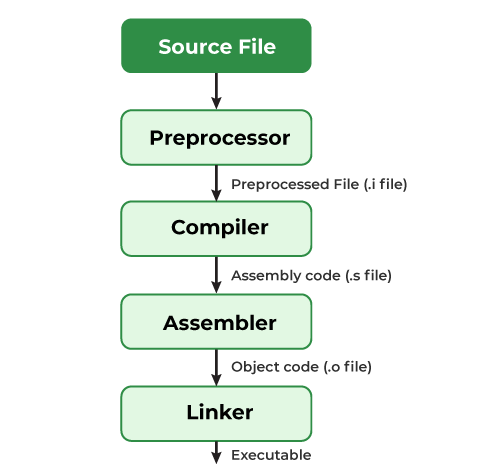
\includegraphics[width=0.35\textheight]
	{assets/pics/program_compile.png}
	\caption{Alur kompilasi program}
\end{figure}

\subsubsection{Proses Eksekusi}
Setelah program dikompilasi menjadi file executable, proses eksekusi dimulai [5]. Proses eksekusi melibatkan beberapa tahapan yang dilakukan oleh sistem operasi:
\begin{enumerate}
	\item \bo{Loading:} Loader yaitu sebuah komponen dari sistem operasi, memuat file executable ke dalam memori utama (RAM). Loader mengalokasikan ruang memori yang dibutuhkan oleh program, memuat instruksi dan data ke dalam memori, dan menginisialisasi program untuk eksekusi.
	\item \bo{Eksekusi:} Setelah program dimuat ke dalam memori, prosesor mulai mengeksekusi instruksi-instruksi yang terdapat dalam program. Prosesor mengambil instruksi satu per satu dari memori, mendekode instruksi, dan mengeksekusinya. Siklus ini berulang hingga program selesai dijalankan atau dihentikan.
	\item \bo{Terminasi:} Program berakhir ketika mencapai instruksi terminasi atau ketika terjadi kesalahan yang menyebabkan program berhenti secara paksa. Sistem operasi kemudian membebaskan sumber daya yang digunakan oleh program, seperti memori dan file.
\end{enumerate}

\begin{figure}
	\centering
	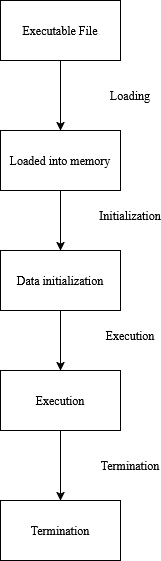
\includegraphics[height=0.5\textheight]
	{assets/pics/program_execution.png}
	\caption{Alur eksekusi program}
\end{figure}

%-----------------------------------------------------------------------------%
\section{\f{Software Control Flow}}
%-----------------------------------------------------------------------------%
Alur kendali perangkat lunak (software control flow) merupakan aspek fundamental dalam eksekusi program, merepresentasikan urutan instruksi yang dieksekusi oleh prosesor untuk mencapai tujuan fungsionalitas program [6]. Memahami  software control flow adalah krusial dalam analisis kode, terutama dalam reverse engineering karena memungkinkan pemetaan jalur eksekusi, identifikasi bottleneck, dan potensi kerentanan. Dalam konteks ini, control flow bukan hanya sekadar urutan instruksi, tetapi juga representasi logis dari bagaimana program merespons input, kondisi, dan interaksi dengan sistem operasi. Pemahaman yang komprehensif terhadap aspek ini memberikan dasar yang kuat dalam menganalisis perilaku program, baik secara statis melalui analisis kode sumber dan intermediate representation, maupun secara dinamis melalui observasi eksekusi runtime.

\subsection{\f{Control Flow Instructions}}
Instruksi alur kendali (control flow instructions) adalah mekanisme fundamental yang menentukan urutan eksekusi instruksi dalam suatu program [6]. Instruksi ini memungkinkan program untuk membuat keputusan, mengulang blok kode, dan melompat ke bagian kode yang berbeda. Cara instruksi-instruksi ini direpresentasikan dan diimplementasikan sangat bergantung pada tingkat bahasa pemrograman yang digunakan. Secara umum, kita membedakan antara bahasa tingkat tinggi dan bahasa tingkat rendah.

\subsubsection{\f{High Level Languages}}
Bahasa pemrograman tingkat tinggi (high-level languages), seperti Python, Java, C++, dan JavaScript, menyediakan abstraksi yang jauh dari detail hardware. Bahasa-bahasa ini fokus pada kemudahan penulisan dan pemahaman kode oleh programmer, dengan menggunakan sintaks yang lebih dekat dengan bahasa manusia. Instruksi control flow dalam bahasa tingkat tinggi diimplementasikan melalui konstruksi yang intuitif, seperti if, else, for, dan while.

\bi{Conditonal Instructions:}

\begin{itemize}
	\item \bi{if statement:} Memungkinkan program membuat keputusan berdasarkan kondisi.
	\item \bi{if-else statement:} Menyediakan jalur alternatif jika kondisi if tidak terpenuhi.
	\item \bi{switch statement:} Memungkinkan percabangan ke banyak kasus.
\end{itemize}

\bi{Loop Instructions:}

\begin{itemize}
	\item \bi{for loop:} Memungkinkan program membuat keputusan berdasarkan kondisi.
	\item \bi{while loop:} Mengeksekusi blok kode selama kondisi tertentu terpenuhi.
\end{itemize}

\bi{Jump Instructions (Indirect - Function Calls):}

\begin{itemize}
	\item \bi{Function call:} Memindahkan kontrol ke fungsi lain dan kembali setelah selesai.
\end{itemize}

\subsubsection{\f{Low Level Languages}}
Bahasa pemrograman tingkat rendah (low-level languages), seperti Assembly language, bekerja lebih dekat dengan hardware. Instruksi-instruksinya langsung dikodekan ke dalam instruksi mesin yang dapat dieksekusi oleh prosesor. Bahasa tingkat rendah memberikan kontrol yang lebih besar atas hardware, tetapi seringkali lebih kompleks dan sulit untuk dipahami oleh manusia. Instruksi control flow pada tingkat ini melibatkan kode operasi (opcode) yang merepresentasikan operasi jump dan perbandingan secara langsung [7]. Dalam bagian ini, contoh akan difokuskan pada bahasa x86 Assembly.

\bi{Conditonal Instructions:}

\begin{itemize}
	\item \bi{cmp (compare):} Membandingkan dua nilai dan mengatur flags (bendera) kondisi.
	\item \bi{jle, jge, je, jne (conditional jumps):} Melompat ke label lain jika flags kondisi memenuhi syarat.
\end{itemize}

\bi{Loop Instructions (Implementasi dengan Conditional Jumps)}
\begin{itemize}
	\item Menggunakan kombinasi instruksi perbandingan, pengurangan counter, dan conditional jump untuk membuat loop.
\end{itemize}

\bi{Jump Instructions (Direct):}
\begin{itemize}
	\item \bi{jmp (unconditional jump):} Lompat ke label tanpa syarat.
\end{itemize}

\bi{Jump Instructions (Indirect - Function Calls):}
\begin{itemize}
	\item \bi{call:} Melompat ke alamat fungsi dan menyimpan alamat return.
	\item \bi{ret:} Mengembalikan control dari fungsi.
\end{itemize}

\subsection{Control Flow Graph}
Graf Alur Kendali (Control Flow Graph atau CFG) adalah representasi grafis dari alur kendali suatu program. CFG memvisualisasikan bagaimana eksekusi program berjalan melalui berbagai blok kode, menggambarkan urutan eksekusi, percabangan, dan perulangan [8]. CFG sangat penting dalam analisis statis kode, reverse engineering, dan optimisasi kode [9]. Dalam CFG, blok dasar (basic blocks) direpresentasikan sebagai simpul (nodes) dan transisi antar blok dasar direpresentasikan sebagai sisi/garis (edges). Contohnya dapat dilihat pada Gambar BAB II TINJAUAN PUSTAKA.5.

\begin{figure}
	\centering
	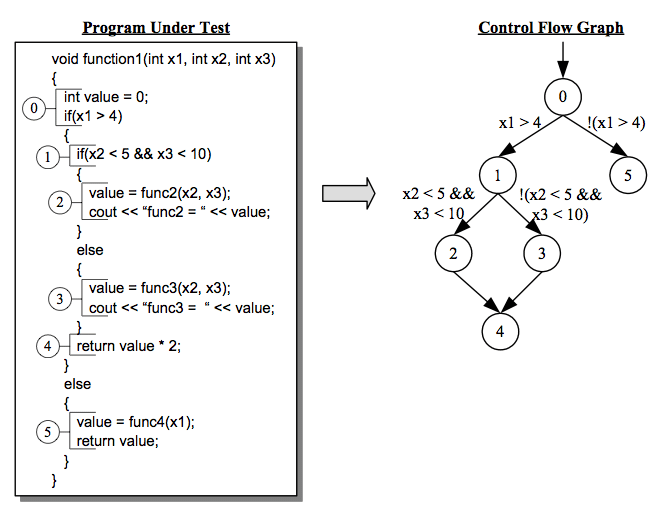
\includegraphics[width=1\textwidth]
	{assets/pics/control_flow_graph.png}
	\caption{Control Flow Graph}
\end{figure}

%-----------------------------------------------------------------------------%
\section{Rekayasa balik (\f{Reverse Engineering})}
%-----------------------------------------------------------------------------%
Rekayasa balik (reverse engineering) adalah proses menganalisis suatu sistem, baik perangkat lunak, perangkat keras, atau sistem lainnya, untuk mengidentifikasi komponen-komponennya dan interaksi antar komponen, serta memahami cara kerja sistem tersebut tanpa akses ke dokumentasi asli atau kode sumber [11]. Tujuannya beragam, mulai dari pemahaman fungsionalitas, analisis keamanan untuk menemukan kerentanan, pemulihan desain, hingga modifikasi dan peningkatan sistem. Rekayasa balik dapat diterapkan pada berbagai skenario, misalnya untuk menganalisis malware, memahami format file yang tidak terdokumentasi, mempelajari teknik yang digunakan oleh pesaing atau modifikasi fungsionalitas perangkat lunak.

\subsection{Jenis Analisis Rekayasa Balik}
\begin{enumerate}
	\item Analisis Statis
	      Analisis statis melibatkan pemeriksaan kode tanpa menjalankannya. Analisis statis berfokus pada struktur dan logika kode, mencari pola dan kerentanan [12]. Alat yang digunakan dalam analisis statis meliputi:
	      \begin{itemize}
		      \item \bi{Disassembler:}  Menerjemahkan kode mesin menjadi assembly code, sebuah representasi kode yang lebih mudah dibaca oleh manusia. Contoh: IDA Pro, Ghidra, Radare2.
		      \item \bi{Decompiler:}  Menerjemahkan kode mesin atau bytecode kembali ke kode sumber tingkat tinggi (misalnya, C++ atau Java). Decompiler membantu memahami logika program secara lebih mudah.
		      \item \bi{Code Analysis Tools:}  Alat yang digunakan untuk menganalisis kode secara otomatis, mencari kerentanan keamanan, pola kode yang buruk, dan masalah lainnya.
	      \end{itemize}

	      \begin{figure}
		      \centering
		      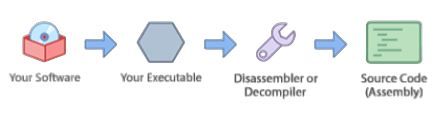
\includegraphics[width=.75\textwidth]
		      {assets/pics/program_decompile.png}
		      \caption{Dekompilasi Aplikasi}
	      \end{figure}
	\item Analisis Dinamik
	      Analisis dinamis melibatkan menjalankan program dan mengamati perilakunya. Analisis dinamis berfokus pada bagaimana program berinteraksi dengan lingkungannya, mencari kerentanan runtime dan memahami alur eksekusi [12]. Alat yang digunakan dalam analisis dinamis meliputi:
	      \begin{itemize}
		      \item \bi{Debugger:} Memungkinkan eksekusi program secara terkontrol, memeriksa nilai variabel, dan melacak alur eksekusi. Contoh: x64dbg, OllyDbg, GDB.
		      \item \bi{Profiler:} Mengukur penggunaan sumber daya program, seperti waktu eksekusi, penggunaan memori, dan akses file. Profiler membantu mengidentifikasi bottleneck kinerja.
	      \end{itemize}
\end{enumerate}

\subsection{\f{Tampering}}
\f{Tampering} merupakan suatu proses mengubah kode aplikasi untuk mempengaruhi perilakunya. Contoh Tampering perangkat lunak adalah mengubah kode aplikasi agar dapat melewati proses autentikasi dalam perangkat lunak tersebut. Hal ini dapat dilakukan dengan memodifikasi control flow pada proses autentikasi dalam programnya. \\
\f{Tampering} bisa dilakukan pada berbagai tingkatan dan bagian dari perangkat lunak, termasuk
\begin{itemize}
	\item \bo{Kode biner (\textit{executable code}):} Mengubah instruksi mesin yang dijalankan oleh prosesor. Hal ini bisa digunakan untuk mematikan fitur tertentu, menambahkan fitur baru, mengubah perilaku program, atau menyisipkan kode berbahaya.
	\item \bo{Data} Mengubah data konfigurasi, aset game, atau data sensitif lainnya yang digunakan oleh program.
	\item \bo{Pustaka (\textit{Library}):} Memodifikasi library yang digunakan oleh program untuk mengubah fungsionalitasnya.
	\item \bo{Sumber Daya (\textit{Resources}):} Mengubah teks, gambar, atau elemen lain yang digunakan oleh program.
\end{itemize}


\subsection{Alat-alat untuk Rekayasa Balik}
\begin{itemize}
	\item \bo{IDA Pro (Interactive Disassembler Pro):} Disassembler dan debugger komersial yang sangat populer dan powerful. IDA Pro mendukung berbagai arsitektur prosesor dan sistem operasi, menyediakan antarmuka yang canggih untuk analisis kode, dan mendukung plugin untuk ekstensibilitas [13].
	      \begin{figure}
		      \centering
		      
\includegraphics[width=.6\textwidth]
		      {assets/pics/IDA_pro.png}
		      \caption{IDA Pro}
	      \end{figure}
	\item \bo{Ghidra:} Framework reverse engineering open-source yang dikembangkan oleh NSA (National Security Agency). Ghidra menawarkan fitur yang setara dengan IDA Pro, termasuk disassembler, decompiler, dan debugger. Ghidra juga mendukung scripting dan ekstensibilitas melalui plugin [14].
	      \begin{figure}
		      \centering
		      
\includegraphics[width=.4\textwidth]
		      {assets/pics/Ghidra.png}
		      \caption{Ghidra}
	      \end{figure}
	\item \bo{x64dbg:} Debugger open-source untuk platform Windows. x64dbg menyediakan antarmuka yang modern dan user-friendly, serta mendukung plugin dan scripting. x64dbg fokus pada analisis malware dan reverse engineering aplikasi Windows. [15]
	      \begin{figure}
		      \centering
		      
\includegraphics[width=.5\textwidth]
		      {assets/pics/x64Dbg.png}
		      \caption{x64dbg}
	      \end{figure}
\end{itemize}

%-----------------------------------------------------------------------------%
\section{\f{Obfuscation}}
%-----------------------------------------------------------------------------%
Obfuscation adalah teknik yang digunakan untuk mengubah kode sumber atau kode mesin menjadi bentuk yang lebih sulit dipahami oleh manusia, tanpa mengubah fungsionalitas program. Tujuan utama obfuscation adalah untuk mempersulit analisis dan reverse engineering, melindungi kekayaan intelektual, dan meningkatkan keamanan aplikasi. Obfuscation tidak membuat kode menjadi tidak mungkin untuk di-reverse engineer, tetapi meningkatkan waktu dan usaha yang dibutuhkan untuk melakukannya, sehingga membuat reverse engineering menjadi kurang menarik bagi penyerang

\subsection{Manfaat \f{Obfuscation}}
\begin{itemize}
	\item \bo{Meningkatkan Keamanan:} Obfuscation mempersulit penyerang untuk memahami logika program, menemukan kerentanan, dan memodifikasi kode untuk tujuan jahat. Obfuscation dapat melindungi algoritma penting, kunci enkripsi, dan data sensitif lainnya.
	\item \bo{Melindungi Kekayaan Intelektual:} Obfuscation dapat mempersulit pesaing untuk mencuri kode sumber, meniru fungsionalitas program, dan melanggar hak cipta. Ini penting terutama untuk perangkat lunak komersial dan aplikasi yang mengandung algoritma atau teknologi yang unik.
\end{itemize}

\subsection{Jenis-jenis \f{Obfuscation}}
Obfuscation dapat dilakukan pada diterapkan pada kode sumber, bytecode, atau kode biner.
\subsubsection{Kode Sumber \f{Obfuscation}}
Teknik ini mengubah kode sumber yang dapat dibaca manusia, sehingga sulit dipahami tanpa memengaruhi fungsinya [16].
\begin{itemize}
	\item \bi{Layout obfuscation:} mengubah tampilan kode.
	      \begin{itemize}
		      \item \bi{Scrabling identifiers [17]:} mengubah nama fungsi dan variabel.
		      \item \bi{Changing formatting [18]:} menambahkan atau menghapus spasi putih dan baris baru.
		      \item \bi{Removing comments [18]:} menghapus komentar penjelasan.
	      \end{itemize}
	\item \bi{Data obfuscation:} menyembunyikan cara data disimpan dan diproses.
	      \begin{itemize}
		      \item \bi{Data encocding [19] [20] [21]:} Mengubah representasi data, misalnya mengenkripsi string atau mengubah nilai numerik dengan operasi matematika. Ini membuat data asli sulit dikenali langsung.
		      \item \bi{Instruction Substitution [22] [23]} Mengganti instruksi yang sederhana dengan instruksi yang lebih kompleks atau setara, tetapi lebih sulit dipahami.
		      \item \bi{Mixed boolean arithmetic [24] [25] [26]} Menggunakan operasi boolean (AND, OR, XOR, NOT) yang dikombinasikan dengan operasi aritmatika untuk membuat logika program lebih kompleks dan sulit diurai.
	      \end{itemize}
	\item \bi{Control flow obfuscation:} mempersulit logika program.
	      \begin{itemize}
		      \item \bi{Bogus control flow [27]:} menambahkan kode palsu yang memengaruhi alur kontrol.
		      \item \bi{Opaque predicates [28]:} menyisipkan kode sampah ke dalam pernyataan kondisional.
		      \item \bi{Control Flow flattening [29]:} mengubah struktur program menjadi pernyataan switch yang kompleks.
	      \end{itemize}
\end{itemize}

\subsubsection{\f{Bytecode Obfuscation}}
Bytecode Obfuscation beroperasi pada kode perantara yang dihasilkan setelah kompilasi kode sumber. Hal ini khususnya relevan untuk bahasa seperti Java, .NET, LLVM dimana kode dikompilasi menjadi bytecode dan kemudian dijalankan pada mesin virtual [30] [31]. Tujuannya adalah untuk mempersulit rekayasa balik bytecode menjadi kode sumber dengan mudah.\\
Berikut Teknik-teknik obfuscation pada bytecode :
\begin{itemize}
	\item \bi{Renaming [30] :} Mengubah nama kelas, metode, dan variabel dalam bytecode untuk membuat kode sumber yang didekompilasi lebih sulit dibaca. Misalnya, metode bernama calculateSalary dapat diubah namanya menjadi method1
	\item \bi{Control Flow Obfucsation [30] :} Meggunakna  percabangan yang kompleks, kondisional, dan konstruksi berulang untuk membuat kode yang didekompilasi menjadi non-deterministik dan lebih sulit untuk diikuti
	\item \bi{String Encryption [30] :} Mengenkripsi string yang tertanam dalam bytecode, yang hanya didekripsi saat dijalankan saat dibutuhkan. Hal ini mempersulit pencarian informasi atau data sensitif dengan menganalisis bytecode.
	\item \bi{Dummy Code Insertion [30] :} Menambahkan kode yang tidak memengaruhi logika program, tetapi mempersulit dekompilasi dan analisis
\end{itemize}

\subsubsection{\f{Kode Biner Obfuscation}}
Kode Biner Obfuscation diterapkan pada kode akhir yang dapat dieksekusi mesin. Ini berfokus pada upaya membuat biner sulit dianalisis, dibongkar, dan dipahami. Berikut beberapa teknik yang digunakna untuk obfuscation pada kode biner :
\begin{itemize}
	\item bi{Code Packing [32] :} kode asli yang dapat dieksekusi dikompresi atau dienkripsi menjadi biner yang dikemas, yang juga menyertakan kode bootstrap yang membongkar kode asli ke dalam memori saat runtime, sehingga melindungi kode asli dari analisis statis.
	\item bi{Obfuscated Control Flow [32] :} Menggunakan inderect calls dan  jumps, dan memanipulasi instruksi panggilan dan ret untuk mempersulit mengikuti jalur eksekusi program.
	\item bi{Chunked Control Flow [32] :} Membagi kode menjadi blok-blok yang sangat kecil dengan instruksi lompatan antar blok untuk mengganggu pembongkaran linear assembly.
	\item bi{Obfuscated Constants [32] :} Menyembunyikan nilai konstan yang digunakan dalam kode melalui berbagai operasi aritmatika atau logika.
	\item bi{Code Virtualization [32] :} Menerjemahkan kode mesin menjadi instruksi virtual yang dieksekusi oleh mesin virtual khusus yang tertanam dalam aplikasi.
\end{itemize}

\begin{figure}
	\centering
	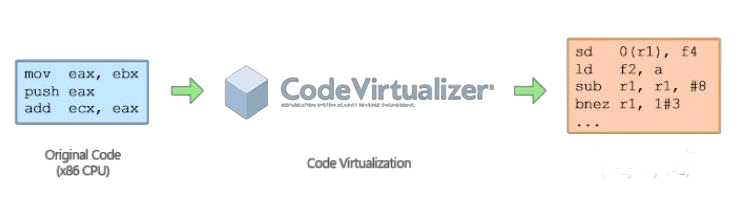
\includegraphics[width=.8\textwidth]
	{assets/pics/code_virtualization_process.png}
	\caption{Prosess Code Virtualization [1]}
\end{figure}
%-----------------------------------------------------------------------------%
\section{\f{Code Virtualization}}
%-----------------------------------------------------------------------------%

Code Virtualization atau juga disebut dengan VM-Based Code Obfuscation menerupakan suatu teknik obfuscation dimana kita menerjemahkan kode biner orignal menjadi bytecode baru berdasarkan Instruction Set Architecture (ISA) khusus (Gambar BAB II TINJAUAN PUSTAKA.10). Bytecode ini dapat dijalankan secara run-time dengan mesin virtual (i.e. intrepreter) yang tertanam pada aplikasinya [33]. Teknik Code virtualization tidak akan mengembalikan sumber kode aslinya dalam memori sedangkan teknik Code Encryption tetap mengembalikan kodenya aslinya dalam memori saat dilakukan dekripsinya [34].

Set instruksi virtual ini merupakan kunci dari obfuscationnya yang digunakan untuk mapping relasi antara intruksi lokal dan instruksi virtual [33]. Intruksi virtual ini membuat aliran kontrol dari original program untuk tidak dapat dibaca dan mempersulit reverse-engineer program. Code Virtualization dapat menghasilkan berbagai mesin virtual dengan set instruksi virtual masing-masing. Dengan ini, setiap copy dari program dapat memiliki instruksi virtual khusus agar mencegah penyerang untuk mengenali opcode mesin virtual menggunakan metode Frequency Analysis [1] [33].

\begin{figure}
	\centering
	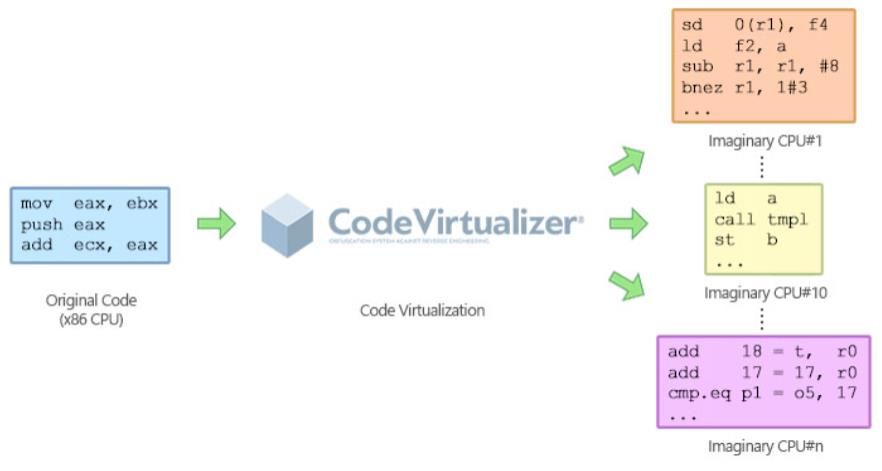
\includegraphics[width=1\textwidth]
	{assets/pics/multiple_virtualization.jpg}
	\caption{Transformasi ISA x86 menjadi berbagai messin virtual [1]}
\end{figure}

Arsitektur umum mesin virtual untuk Code Virtualization memiliki komponen-komponen yang mirip dengan design CPU [35] [36]
\begin{enumerate}
	\item \bi{VM entry:} Perannya untuk simpan konteks eksekusi native (seperti register CPU atau flag) dan transisi ke konteks mesin virtual.
	\item \bi{Fetch:} Perannya adalah untuk mengambil, dari memori internal VM, opcode (virtual) yang akan ditiru, berdasarkan nilai Virtual Program Counter (vpc).
	\item \bi{Decode:} Perannya adalah untuk mendekode opcode yang diambil dan operan yang sesuai untuk menentukan instruksi ISA mana yang akan dieksekusi.
	\item \bi{Dispatch:} Setelah instruksi didekodekan, operator menentukan pengendali mana yang harus dijalankan dan mengatur konteksnya.
	\item \bi{Handlers:} Meniru instruksi virtual melalui rangkaian instruksi asli dan memperbarui konteks internal VM, biasanya vpc.
	\item \bi{VM exit:} Perannya untuk transisi dari konteks mesin virtual balik ke konteks eksekusi native.
\end{enumerate}

Proses eksekusi Code Virtualization pada program dapat dilihat pada Gambar BAB II TINJAUAN PUSTAKA.12 dan contoh code virtualization pada intel assembly dapat dilihat pada Gambar BAB II TINJAUAN PUSTAKA.13.

\begin{figure}
	\centering
	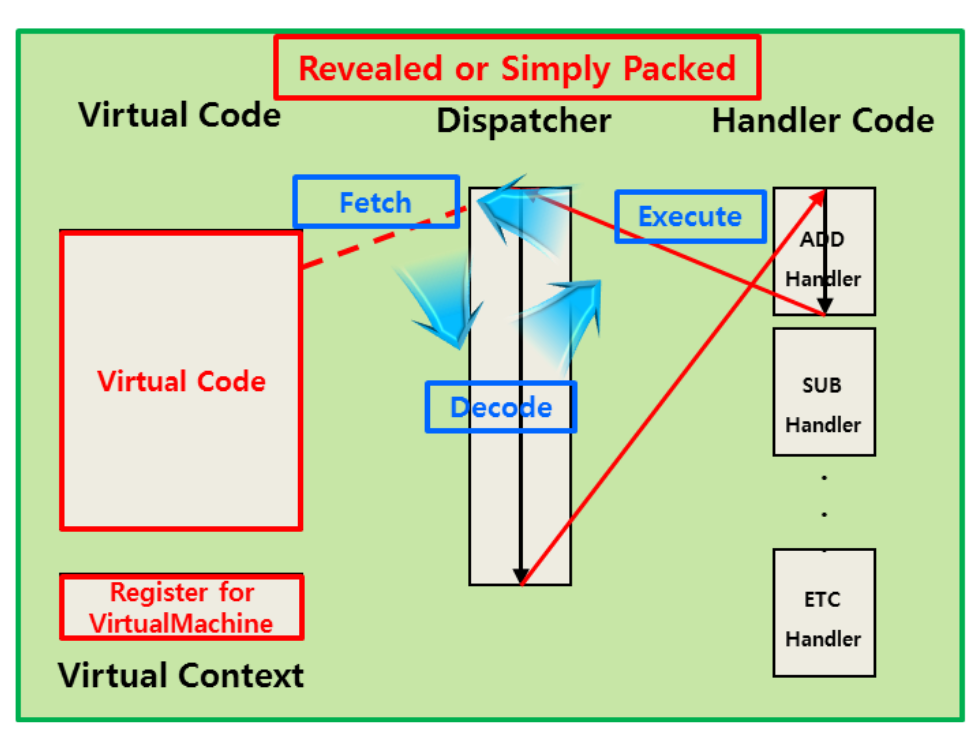
\includegraphics[width=0.7\textwidth]
	{assets/pics/virtualization_execution.png}
	\caption{Alur eksekusi Code Virtualization [34]}
\end{figure}

\begin{figure}
	\centering
	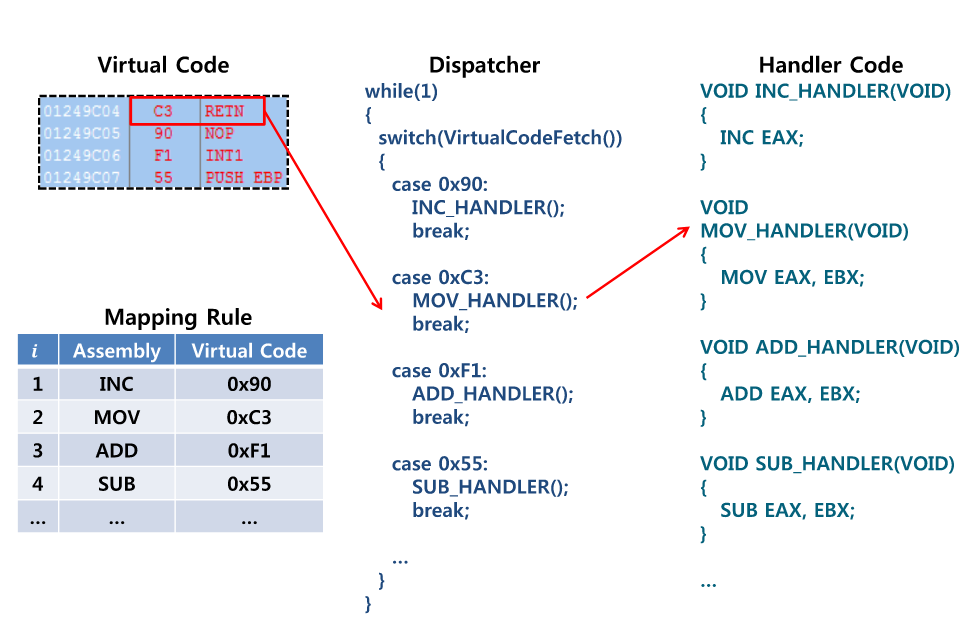
\includegraphics[width=0.7\textwidth]
	{assets/pics/code_to_virtualized.png}
	\caption{Transformasi kode asli menjadi kode virtual [34]}
\end{figure}

\subsection{EagleVM}
EagleVM adalah implementasi code virtualization open-source untuk arsitektur x86-64 yang dirancang khusus untuk tujuan penelitian dan demonstrasi [2]. Proyek ini merupakan hasil kompilasi penelitian dari Code Virtualizer komersial seperti VMProtect, Themida, dan Enigma Protector [1] [37] [38]. Proyek ini berfokus pada transformasi biner-ke-biner (bin2bin), memungkinkan modifikasi langsung pada file executable tanpa memerlukan akses ke kode sumber. EagleVM menyediakan kerangka kerja yang fleksibel untuk mempelajari dan mengembangkan teknik virtualisasi kode, serta menawarkan kemampuan untuk melindungi bagian-bagian tertentu dari kode program dari analisis reverse-engineering. Meskipun bersifat open-source dan bermanfaat untuk riset, EagleVM tidak didesain untuk penggunaan produksi dan memiliki keterbatasan dalam hal stabilitas dan fitur.

\subsubsection{Komponen EagleVM}
EagleVM memiliki arsitektur modular yang terdiri dari beberapa komponen yang bekerja sama [2]:
\begin{itemize}
	\item \bo{EagleVM (Core):} Inti dari EagleVM, berisi logika utama untuk memproses biner input, melakukan disassembly, menerjemahkan instruksi x86-64 ke bytecode, dan menghasilkan biner output yang mengandung mesin virtual dan bytecode. Komponen ini juga bertanggung jawab untuk mengelola konteks eksekusi, termasuk pemetaan register dan stack.
	\item \bo{EagleVM.Stub:} Dynamic Link Library (DLL) yang berperan penting dalam proses penandaan kode yang akan divirtualisasi. DLL ini mengekspor dua fungsi utama, yaitu fnEagleVMBegin dan fnEagleVMEnd. Pengembang menggunakan fungsi-fungsi ini di dalam kode sumber mereka untuk menandai awal dan akhir blok kode yang akan dilindungi dengan virtualisasi. EagleVM kemudian akan mencari panggilan ke fungsi-fungsi ini dalam biner input untuk mengidentifikasi bagian kode yang harus divirtualisasi.
	\item \bo{EagleVM.Sandbox:} Sebuah aplikasi contoh yang berfungsi sebagai sandbox untuk mendemonstrasikan cara menggunakan EagleVM dan EagleVM.Stub. Proyek ini memberikan contoh konkret tentang bagaimana mengintegrasikan EagleVM ke dalam alur kerja pengembangan perangkat lunak dan bagaimana memanfaatkan fitur-fitur yang disediakan oleh EagleVM.Stub untuk menandai kode yang akan divirtualisasi.
\end{itemize}

\subsubsection{Arsitektur Mesin Virtual EagleVM}
Mesin virtual EagleVM didesain dengan mempertimbangkan kesederhanaan dan kemudahan implementasi, sambil tetap memberikan perlindungan yang memadai terhadap reverse engineering. Arsitekturnya menyerupai arsitektur CPU sederhana, dengan komponen-komponen utama sebagai berikut:
\begin{itemize}
	\item \bo{Konteks x86-64 dan VM:} Saat memasuki mesin virtual, konteks x86-64 asli (nilai register dan stack pointer) disimpan di stack. EagleVM kemudian mengalokasikan ruang di stack untuk konteks mesin virtual, termasuk register virtual dan virtual call stack. Register R0-R15 x86-64 kemudian dapat digunakan oleh mesin virtual. Dokumentasi EagleVM menyebutkan bahwa register RFLAGS selalu disimpan pertama di stack karena otomatisasi dalam pembuatan VMENTER dan VMEXIT.
	\item \bo{Register Virtual} EagleVM menggunakan sejumlah register virtual untuk eksekusi bytecode. Beberapa register virtual yang penting meliputi:
	      \begin{itemize}
		      \item VIP (Virtual Instruction Pointer): Analog dengan RIP pada x86-64, menunjuk ke instruksi virtual selanjutnya yang akan dieksekusi.
		      \item VSP (Virtual Stack Pointer): Analog dengan RSP pada x86-64, menunjuk ke puncak stack virtual.
		      \item VREGS: Penunjuk ke awal area di stack yang menyimpan nilai register x86-64 yang disimpan.
		      \item VCS (Virtual Call Stack): Digunakan untuk menyimpan alamat kembali (return address) saat panggilan fungsi virtual.
		      \item VTEMP dan VTEMP2: Register sementara untuk perhitungan.
		      \item VCSRET: Menyimpan RVA yang digunakan dalam perhitungan VIP. Pemetaan register virtual ke register x86-64 dilakukan secara acak untuk mempersulit analisis.
	      \end{itemize}
	\item \bo{Virtual Call Stack (VCS):} EagleVM menggunakan virtual call stack untuk mendukung panggilan fungsi di dalam kode yang divirtualisasi. VCS menyimpan alamat kembali ke instruksi setelah panggilan fungsi, memungkinkan mesin virtual untuk melanjutkan eksekusi dengan benar setelah fungsi selesai.
	\item \bo{Handler Instruksi:} Setiap instruksi virtual memiliki handler yang berisi kode x86-64 untuk mengeksekusi instruksi tersebut. Handler inilah yang sebenarnya melakukan operasi yang ditentukan oleh instruksi virtual. EagleVM menyediakan handler untuk berbagai instruksi x86-64, dan pengembang dapat menambahkan handler baru untuk mendukung instruksi lain atau mengimplementasikan perilaku khusus.
	\item \bo{VMENTER dan VMEXIT:} VMENTER bertanggung jawab untuk memasuki lingkungan mesin virtual, menyimpan konteks x86-64, menginisialisasi konteks VM, dan memulai eksekusi bytecode. VMEXIT bertanggung jawab untuk keluar dari lingkungan mesin virtual, memulihkan konteks x86-64, dan mengembalikan kontrol ke kode asli.
\end{itemize}

\subsubsection{Alur Kerja Virtualisasi dengan EagleVM}
Proses virtualisasi kode dengan EagleVM melibatkan langkah-langkah berikut:
\begin{enumerate}
	\item \bo{Penandaan Kode Target:} Pengembang memasukkan panggilan ke fungsi fnEagleVMBegin dan fnEagleVMEnd dari EagleVM.Stub di dalam kode sumber mereka untuk menandai blok kode yang akan divirtualisasi.
	\item \bo{Kompilasi dan Linking:} Kode sumber dikompilasi dan di-link untuk menghasilkan file executable.
	\item \bo{Pemrosesan oleh EagleVM:} File executable yang dihasilkan kemudian diproses oleh EagleVM. EagleVM akan memparsing file executable, mencari panggilan ke fungsi penanda dari EagleVM.Stub, dan mengekstrak kode yang ditandai untuk divirtualisasi.
	\item \bo{Disassembly dan Analisis Alur Kontrol:} EagleVM melakukan disassembly pada kode yang akan divirtualisasi dan membangun representasi alur kontrol program dalam bentuk basic blocks. Analisis ini penting untuk memastikan bahwa alur eksekusi kode yang divirtualisasi tetap sama dengan kode aslinya.
	\item \bo{Transformasi ke Bytecode dan Pembuatan VM:} EagleVM menerjemahkan instruksi x86-64 asli ke dalam bytecode khusus untuk mesin virtualnya. EagleVM juga menghasilkan kode untuk mesin virtual yang akan mengeksekusi bytecode tersebut.
	\item \bo{Pembuatan Biner Output:} EagleVM menghasilkan biner output yang telah dimodifikasi, mengandung bytecode dan mesin virtual.
	\item \bo{Eksekusi:} Saat program dijalankan, mesin virtual yang tertanam dalam biner akan mengambil dan mengeksekusi bytecode, mereplikasi fungsionalitas dari kode asli.
\end{enumerate}

%-----------------------------------------------------------------------------%
\chapter{\babTiga}
%-----------------------------------------------------------------------------%

%-----------------------------------------------------------------------------%
\section{Desain Penelitian}
%-----------------------------------------------------------------------------%
Penelitian ini menggunakan pendekatan eksperimental untuk menganalisis efektivitas code virtualization menggunakan VxLang dalam meningkatkan keamanan perangkat lunak dengan mempersulit reverse engineering. Fokus utama dari eksperimen ini adalah pada pengujian fungsionalitas autentikasi dan analisis performance overhead yang disebabkan oleh penerapan VxLang pada berbagai jenis aplikasi. Dua percobaan utama akan dilakukan:

\begin{enumerate}
	\item \bo{Pengujian Autentikasi - Analisis Statis dan Dinamis:} Percobaan ini bertujuan untuk menganalisis kompleksitas control flow program sebelum dan sesudah di-obfuscate menggunakan VxLang pada tiga jenis aplikasi yang berbeda:
	      \begin{itemize}
		      \item \bo{Aplikasi Konsol (Tanpa GUI) :} Aplikasi sederhana yang berinteraksi melalui command line.
		      \item \bo{Aplikasi Qt :} Aplikasi dengan antarmuka pengguna grafis yang dibangun menggunakan Qt Framework.
		      \item \bo{Aplikasi ImGUI :} Aplikasi dengan antarmuka pengguna grafis yang menggunakan library Dear ImGUI.
	      \end{itemize}
	      Analisis akan dilakukan melalui dua pendekatan: analisis statis menggunakan Ghidra dan analisis dinamis menggunakan x64Dbg. Selain itu, percobaan ini juga akan mencakup upaya untuk melewati pengujian autentikasi dengan memanipulasi control flow menggunakan Ghidra dan x64dbg pada ketiga jenis aplikasi tersebut. Tujuan dari pengujian pada berbagai aplikasi ini adalah untuk menunjukkan bahwa VxLang dapat diterapkan pada berbagai framework dan jenis kode sumber yang berbeda.
	\item \bo{Pengujian Performa - Waktu Eksekusi dan Ukuran File:} Percobaan ini bertujuan untuk mengukur performa waktu eksekusi program dengan algoritma sorting sebelum dan sesudah di-obfuscate, serta membandingkan ukuran file executable. Waktu eksekusi diukur menggunakan library chrono::high\_resolution\_clock.
\end{enumerate}
%-----------------------------------------------------------------------------%
\section{Alat dan Bahan}
%-----------------------------------------------------------------------------%
Perangkat lunak dan perangkat keras yang digunakan dalam penelitian ini adalah:

\begin{itemize}
	\item \bo{Perangkat Lunak:}
	      \begin{itemize}
		      \item \bo{Sistem Operasi:} Windows 11 akan digunakan sebagai lingkungan operasi utama untuk melakukan semua percobaan.
		      \item \bo{Kompiler:} Kompiler Clang (clang-cl) akan digunakan untuk mengkompilasi kode sumber
		      \item \bo{Framwork GUI:} Qt Framework dan Dear ImGUI
		      \item \bo{Alat Virtualisasi Kode:} VxLang akan digunakan sebagai alat utama untuk mengimplementasikan virtualisasi kode.
		      \item \bo{Alat Analisis Statis:} Ghidra, sebuah framework reverse engineering yang dikembangkan oleh NSA, akan digunakan untuk melakukan analisis statis.
		      \item \bo{Alat Analisis Dinamis:} x64dbg, sebuah debugger sumber terbuka untuk Windows, akan digunakan untuk analisis dinamis
		      \item \bo{Pustaka C++:} Pustaka chrono akan digunakan untuk mengukur waktu eksekusi dan OpenSSL untuk melakukan enkripsi AES.
	      \end{itemize}
	\item \bo{Perangkat Lunak:}
	      \begin{itemize}
		      \item \bo{Prosesor:} Intel Core i7-12700H
		      \item \bo{RAM:} 32 GB
	      \end{itemize}
\end{itemize}

%-----------------------------------------------------------------------------%
\section{Prosedur Penelitian}
%-----------------------------------------------------------------------------%
\subsection{Pengujian Autentikasi: Analisis Statis dan Dinamis}
Pengujian autentikasi bertujuan untuk mengevaluasi efektivitas virtualisasi kode dalam menghambat upaya reverse engineering dengan menganalisis aspek statis dan dinamis dari perangkat lunak sebelum dan sesudah obfuscation, serta mencoba untuk melewati mekanisme autentikasi.

Berikut persiapan yang akan dilakukan :
\begin{enumerate}
	\item \bo{Pengaturan Lingkungan:} Lingkungan perangkat lunak diatur untuk memastikan bahwa semua alat (Windows 11, Clang, VxLang, Ghidra, dan x64dbg) serta framework dan library GUI (Qt dan Dear ImGUI) terinstal dan terkonfigurasi dengan benar. Kode sumber aplikasi studi kasus (konsol, Qt, dan Dear ImGUI) disiapkan untuk kompilasi.
	\item \bo{Kompilasi Aplikasi Asli:} Setiap aplikasi studi kasus (konsol, Qt, dan Dear ImGUI) dikompilasi tanpa menerapkan teknik obfuscation apa pun menggunakan kompiler Clang. Hasilnya adalah file executable asli untuk setiap jenis aplikasi.
	\item \bo{Kompilasi Aplikasi yang di-Obfuscate:} Kode sumber aplikasi studi kasus dimodifikasi untuk menyertakan penanda VL\_VIRTUALIZATION\_BEGIN dan VL\_VIRTUALIZATION\_END untuk menunjukkan blok kode yang akan divirtualisasikan. Kode sumber yang dimodifikasi dikompilasi dengan kompiler Clang, dan selanjutnya, executable diproses dengan VxLang untuk menghasilkan versi yang di-obfuscate yang menyertakan mesin virtual dan bytecode yang sesuai.
\end{enumerate}

\begin{figure}
	\centering
	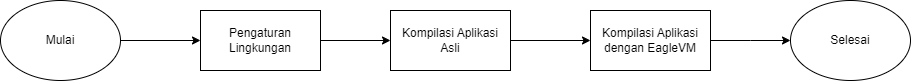
\includegraphics[width=1\textwidth]
	{assets/pics/Persiapan.png}
	\caption{Flow Diagram Persiapan Penelitian}
\end{figure}

\subsubsection{Analisis Statis (Ghidra)}
Fase ini bertujuan untuk menganalisis struktur dan kompleksitas kode tanpa menjalankannya.
\begin{enumerate}
	\item \bo{Peluncuran Ghidra:} Framework Ghidra diluncurkan, dan proyek baru dibuat untuk menampung analisis setiap versi aplikasi (asli dan di-obfuscate untuk konsol, Qt, dan Dear ImGUI).
	\item \bo{Mengimpor Executable:} Baik file executable asli maupun yang di-obfuscate diimpor ke dalam proyek Ghidra.
	\item \bo{Analisis Fungsi:} Fungsi yang menangani proses autentikasi dalam setiap aplikasi dipilih untuk analisis terfokus. Alat analisis Ghidra digunakan untuk membongkar fungsi target dan menghasilkan Control Flow Graph (CFG) untuk kedua versi (obfuscated dan non-obfuscated) dari setiap jenis aplikasi.
	\item \bo{Perbandingan CFG:} CFG dari versi asli dan yang di-obfuscate dibandingkan dengan mendokumentasikan jumlah basic block, edge, dan kompleksitas siklomatik. Kompleksitas siklomatik yang lebih tinggi berkorelasi dengan peningkatan kesulitan dalam pemahaman kode dan reverse engineering. Dokumentasi untuk setiap versi akan mencakup yang berikut:
	      \begin{itemize}
		      \item \bo{Jumlah Basic Block:} Ini menunjukkan jumlah total urutan kode non-percabangan dalam alur kontrol fungsi.
		      \item \bo{Jumlah Edge:} Ini mewakili alur eksekusi dari satu blok ke blok lainnya.
		      \item \bo{Kompleksitas Siklomatik:} Metrik ini mengukur jumlah jalur independen dalam alur kontrol kode. Ini dihitung berdasarkan rumus: Edge - Node + 2
	      \end{itemize}
	\item \bo{Mendokumentasikan Temuan:} Catatan dan observasi terperinci mengenai analisis statis kode dipelihara.
\end{enumerate}

\begin{figure}
	\centering
	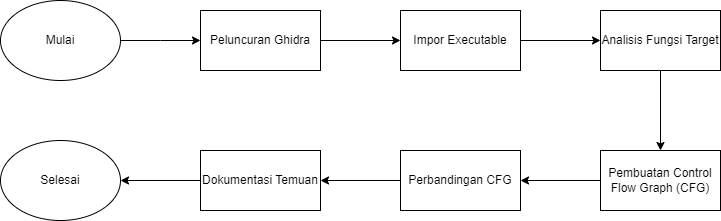
\includegraphics[width=1\textwidth]
	{assets/pics/Static.png}
	\caption{Flow Diagram Analisis Statis}
\end{figure}

\bo{Upaya Manipulasi Control Flow:}
\begin{enumerate}
	\item \bo{Identifikasi Mekanisme Autentikasi:} Menggunakan Ghidra, identifikasi bagian kode yang menangani proses autentikasi. Ini melibatkan pencarian fungsi yang memvalidasi kredensial atau memeriksa lisensi.
	\item \bo{Analisis Control Flow:} Analisis control flow dari fungsi autentikasi untuk memahami bagaimana keputusan autentikasi dibuat.
	\item \bo{Identifikasi Peluang Manipulasi:} Cari peluang untuk memodifikasi control flow (misalnya, mengubah jump kondisional) yang dapat menyebabkan aplikasi selalu menganggap autentikasi berhasil.
	\item \bi{Patching Executable:} Jika memungkinkan, coba patch executable asli menggunakan Ghidra untuk melewati mekanisme autentikasi pada setiap jenis aplikasi.
	\item \bo{Uji Coba Aplikasi yang di-Patch:} Jalankan aplikasi yang di-patch untuk memverifikasi apakah upaya melewati autentikasi berhasil.
	\item \bo{Ulangi pada Aplikasi yang di-Obfuscate:} Lakukan langkah yang sama pada versi aplikasi yang di-obfuscate untuk melihat apakah virtualisasi kode mempersulit upaya manipulasi control flow untuk melewati autentikasi pada setiap jenis aplikasi.
\end{enumerate}

\subsubsection{Analisis Dinamis (x64dbg)}
Analisis dinamis melibatkan pengamatan perilaku program saat dijalankan.
\begin{enumerate}
	\item \bo{Peluncuran x64Dbg:} Debugger x64dbg diluncurkan, dan executable asli dan yang di-obfuscate (untuk konsol, Qt, dan Dear ImGUI) dimuat untuk analisis.
	\item \bo{Pengamatan Alur Eksekusi Autentikasi:} Breakpoint diatur pada fungsi autentikasi untuk mengamati alur eksekusi dan nilai variabel yang relevan selama proses autentikasi pada setiap jenis aplikasi.
	\item \bo{Analisis Perbedaan Alur Kontrol:} Bandingkan alur kontrol eksekusi fungsi autentikasi antara versi asli dan yang di-obfuscate untuk setiap jenis aplikasi. Perhatikan bagaimana virtualisasi kode mengubah urutan instruksi dan mempersulit pemahaman alur kontrol yang sebenarnya.
	\item \bo{Upaya Melewati Autentikasi:} Gunakan x64dbg untuk mencoba memanipulasi alur eksekusi atau nilai variabel selama runtime dengan tujuan untuk melewati mekanisme autentikasi pada setiap jenis aplikasi. Misalnya, coba ubah hasil perbandingan password agar selalu bernilai benar.
	\item \bo{Dokumentasi Temuan:} Catat semua observasi, termasuk kesulitan dalam memahami alur kontrol dan keberhasilan atau kegagalan upaya melewati autentikasi pada setiap jenis aplikasi.
\end{enumerate}

\begin{figure}
	\centering
	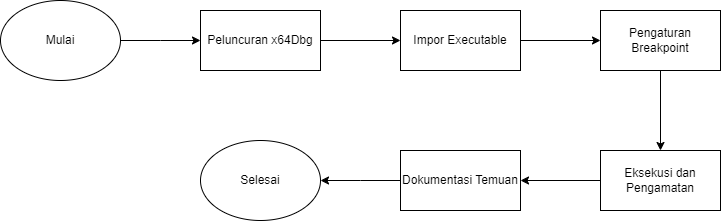
\includegraphics[width=1\textwidth]
	{assets/pics/Dynamic.png}
	\caption{Flow Diagram Analisis Dinamis}
\end{figure}

\subsection{Pengujian Performa: Waktu Eksekusi dan Ukuran File}
Pengujian kinerja ini bertujuan untuk mengevaluasi dampak virtualisasi kode terhadap waktu eksekusi dan ukuran file aplikasi. Untuk mendapatkan pengukuran yang komprehensif, kita akan menggunakan algoritma pengurutan (sorting) sebagai benchmark.

Berikut persiapan yang akan dilakukan :
\begin{enumerate}
	\item \bo{Pemilihan Algoritma Pengurutan:} Algoritma pengurutan yang akan digunakan sebagai benchmark adalah algoritma pengurutan cepat (Quicksort). Quicksort dipilih karena efisiensinya yang baik dalam banyak kasus, serta kompleksitasnya yang cukup untuk memberikan gambaran yang baik tentang performa.
	\item \bo{Pengembangan Benchmark:} Benchmark akan diimplementasikan dengan membuat fungsi yang melakukan pengurutan pada array data. Array data akan diisi dengan angka acak untuk memastikan pengujian yang representatif. Ukuran array data akan divariasikan (misalnya, 1000, 10000, 100000 elemen) untuk mengamati performa pada berbagai skala data.
	\item \bo{Integrasi Benchmark:} Fungsi benchmark diintegrasikan ke dalam kedua versi aplikasi (asli dan yang di-obfuscate). Hal ini memungkinkan kita untuk mengukur waktu eksekusi dari algoritma pengurutan pada kedua versi aplikasi secara terpisah.
\end{enumerate}

\subsubsection{Pengukuran Waktu Eksekusi Enskripsi AES}
\begin{enumerate}
	\item \bo{Benchmark:} Fungsi benchmark akan melakukan enkripsi AES-CBC-256 pada 1 Gigabyte blok.
	\item \bo{Pengukuran Waktu:} Pustaka chrono::high\_resolution\_clock dari C++ akan digunakan untuk mengukur secara akurat waktu yang dibutuhkan untuk setiap eksekusi benchmark.
	\item \bo{Pencatatan Data:} Waktu eksekusi setiap run (dalam milidetik atau mikrosekon) dicatat untuk setiap ukuran array pada kedua versi aplikasi.
\end{enumerate}

\subsubsection{Pengukuran Waktu Eksekusi Quick Sort}
\begin{enumerate}
	\item \bo{Eksekusi Benchmark:} Fungsi benchmark (algoritma pengurutan) akan dieksekusi beberapa kali (misalnya, N=100) pada setiap ukuran array untuk mendapatkan data yang cukup.
	\item \bo{Pengukuran Waktu:} Pustaka chrono::high\_resolution\_clock dari C++ akan digunakan untuk mengukur secara akurat waktu yang dibutuhkan untuk setiap eksekusi benchmark.
	\item \bo{Pencatatan Data:} Waktu eksekusi setiap run (dalam milidetik atau mikrosekon) dicatat untuk setiap ukuran array pada kedua versi aplikasi.
	\item \bo{Perhitungan Rata-Rata:} Waktu eksekusi rata-rata dihitung untuk setiap versi dan setiap ukuran array dengan menjumlahkan semua waktu eksekusi dan membaginya dengan jumlah run (N).
\end{enumerate}

\subsubsection{Pengukuran Ukuran File}
\begin{enumerate}
	\item \bo{Perbandingan Ukuran File:} Ukuran file dari executable asli dan yang di-obfuscate dibandingkan untuk menentukan dampak virtualisasi kode pada ukuran aplikasi.
\end{enumerate}

\begin{figure}
	\centering
	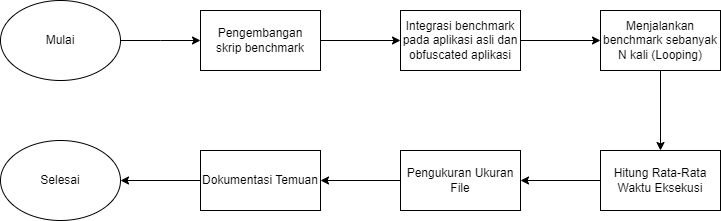
\includegraphics[width=1\textwidth]
	{assets/pics/Performance.png}
	\caption{Flow Diagram Analisis Performa}
\end{figure}

\section{Teknik Analisis Data}
Data yang dikumpulkan dari kedua rangkaian percobaan akan dianalisis menggunakan teknik deskriptif dan komparatif.
\subsection{Analisis Data Pengujian Autentikasi}
\begin{itemize}
	\item \bo{Analisis Data Statis:} Metrik kompleksitas yang diperoleh dari analisis statis (yaitu, jumlah basic block, edge, dan kompleksitas siklomatik) akan dievaluasi. Perbedaan akan digunakan untuk menilai efektivitas virtualisasi kode.
	\item \bo{Analisis Data Dinamis:} Hasil dari analisis dinamis, termasuk alur eksekusi yang diamati dan kesulitan dalam analisis kode, akan dianalisis.
	\item \bo{Evaluasi Efektivitas Keamanan:} Hasil dari analisis dinamis, termasuk alur eksekusi yang diamati dan kesulitan dalam analisis kode, akan dianalisis.
\end{itemize}

\subsection{Analisis Data Pengujian Performa}
\begin{itemize}
	\item \bo{Perbandingan Waktu Eksekusi:} Waktu eksekusi rata-rata antara aplikasi asli dan yang di-obfuscate dibandingkan untuk menilai potensi overhead kinerja yang diperkenalkan oleh VxLang.
	\item \bo{Perbandingan Ukuran File:} Ukuran file dari kedua versi dibandingkan untuk menilai dampak ukuran file dari virtualisasi kode.
	\item \bo{Analisis Trade-off:} Analisis komprehensif dilakukan untuk mengevaluasi trade-off antara keamanan dan kinerja, berdasarkan temuan.
\end{itemize}

%-----------------------------------------------------------------------------%
\chapter{\babEmpat}
%-----------------------------------------------------------------------------%
Bab ini menyajikan penjabaran mendalam mengenai realisasi teknis dari metodologi penelitian yang telah diuraikan pada Bab 3. Fokus utama adalah pada langkah-langkah konkret yang diambil untuk membangun lingkungan eksperimen, mengembangkan artefak perangkat lunak yang diuji, dan mengaplikasikan teknik \f{code virtualization} menggunakan platform VxLang. Pembahasan mencakup detail penyiapan lingkungan, arsitektur aplikasi studi kasus, implementasi \f{benchmark} performa, dan proses integrasi VxLang itu sendiri.

%-----------------------------------------------------------------------------%
\section{Penyiapan Lingkungan Pengembangan}
%-----------------------------------------------------------------------------%
Fondasi dari penelitian eksperimental ini adalah lingkungan pengembangan yang konsisten dan terdefinisi dengan baik. Hal ini krusial untuk memastikan reliabilitas dan reproduktifitas hasil. Komponen-komponen kunci yang dikonfigurasi adalah sebagai berikut:

\begin{itemize}
    \item \bo{Sistem Operasi:} Seluruh proses pengembangan, kompilasi, dan eksekusi pengujian dilakukan pada \bo{Microsoft Windows 11 (64-bit)}. Pemilihan Windows sebagai platform utama didasarkan pada target \f{executable} PE (Portable Executable) yang umum didukung oleh \f{tool} proteksi perangkat lunak seperti VxLang.
    \item \bo{Compiler:} \bo{Clang} (versi 19.1.3), diakses melalui antarmuka \bo{\code{clang-cl}}, dipilih sebagai \f{compiler} C++. Penggunaan \code{clang-cl} memastikan kompatibilitas biner dengan toolchain Microsoft Visual C++ (MSVC), yang seringkali menjadi prasyarat atau lingkungan yang didukung optimal oleh VxLang, sambil tetap memanfaatkan kemampuan analisis dan optimasi modern dari Clang. Proyek ini dikompilasi dengan standar bahasa \bo{C++17}.
    \item \bo{Build System \& Generator:} \bo{CMake} (versi 3.31) digunakan sebagai \f{meta-build system} untuk mengelola kompleksitas \f{build} lintas target dan dependensi. File \code{CMakeLists.txt} mendefinisikan target-target \f{build}, dependensi, dan opsi kompilasi. \bo{Ninja} (versi 1.12.1) digunakan sebagai \f{build generator} di bawah CMake untuk mempercepat proses kompilasi paralel. Konfigurasi \code{CMAKE\_EXPORT\_COMPILE\_COMMANDS} diaktifkan untuk memfasilitasi integrasi dengan \f{tool} analisis kode.
    \item \bo{Integrated Development Environment (IDE):} Neovim dengan LSP Clangd digunakan untuk efisiensi dalam penulisan kode, navigasi, dan \f{debugging} awal.
    \item \bo{Manajemen Dependensi \& Library Pihak Ketiga:} Library eksternal dikelola secara manual dengan menempatkan \f{header} di direktori \code{includes} dan \code{deps}, serta file library (\code{.lib}) di direktori \code{lib}. Library utama yang digunakan meliputi:
          \begin{itemize}
              \item \bo{VxLang SDK:} Terdiri dari file \f{header} (\code{includes/vxlang/vxlib.h}) yang mendefinisikan makro penanda virtualisasi (\code{VL\_VIRTUALIZATION\_BEGIN}, \code{VL\_VIRTUALIZATION\_END}) dan library statis (\code{lib/vxlib64.lib}) yang diperlukan oleh proses virtualisasi.
              \item \bo{Qt Framework:} Versi \bo{6.\textit{x}} (MSVC 2022 64-bit) diintegrasikan menggunakan \code{find\_package(Qt6)} CMake. Modul \code{Widgets} digunakan untuk komponen GUI.
              \item \bo{Dear ImGui:} Library Dear ImGui beserta \f{backend} \bo{GLFW} dan \bo{OpenGL3} di-\f{compile} sebagai bagian dari proyek (\code{deps/*.cpp}).
              \item \bo{libcurl:} Digunakan untuk komunikasi HTTP pada aplikasi autentikasi varian \f{cloud}.
              \item \bo{OpenSSL:} Versi \bo{3.\textit{x}} (\code{libssl}, \code{libcrypto}) digunakan untuk implementasi enkripsi AES pada \f{benchmark} performa.
              \item \bo{nlohmann/json:} Library C++ \f{header-only} untuk menangani data JSON pada varian \f{cloud}.
          \end{itemize}
\end{itemize}

%-----------------------------------------------------------------------------%
\section{Implementasi Pengujian Autentikasi}
%-----------------------------------------------------------------------------%
Bagian ini berfokus pada pengembangan aplikasi yang mensimulasikan proses login pengguna, yang kemudian menjadi subjek analisis \f{reverse engineering} sebelum dan sesudah penerapan VxLang. Pendekatan analisis mencakup analisis statis menggunakan Ghidra dan analisis dinamis menggunakan x64dbg, keduanya bertujuan mengidentifikasi dan mencoba mem-\textit{bypass} logika autentikasi.

Diagram alur persiapan \f{executable} disajikan pada Gambar \ref{fig:flow_auth_prep_rev}. Proses analisis statis dan dinamis, termasuk upaya \textit{bypass}, diilustrasikan pada Gambar \ref{fig:flow_auth_analysis_rev}. Analisis dinamis dimulai dengan langkah serupa analisis statis, yaitu mencari \textit{string} atau pola kode yang relevan di dalam \textit{debugger} (x64dbg) untuk membantu menemukan lokasi logika autentikasi. Setelah lokasi potensial ditemukan, \textit{breakpoint} dipasang. Upaya \textit{bypass} kemudian dilakukan baik secara statis (mem-\textit{patch} file \textit{executable} menggunakan Ghidra) maupun secara dinamis (mem-\textit{patch} instruksi \textit{jump} kondisional atau memanipulasi register/memori secara langsung di x64dbg saat program berjalan).

%--- DIAGRAM PERSIAPAN AUTH ---
\begin{figure}[htbp]
    \centering
    % Menggunakan scale daripada resizebox
    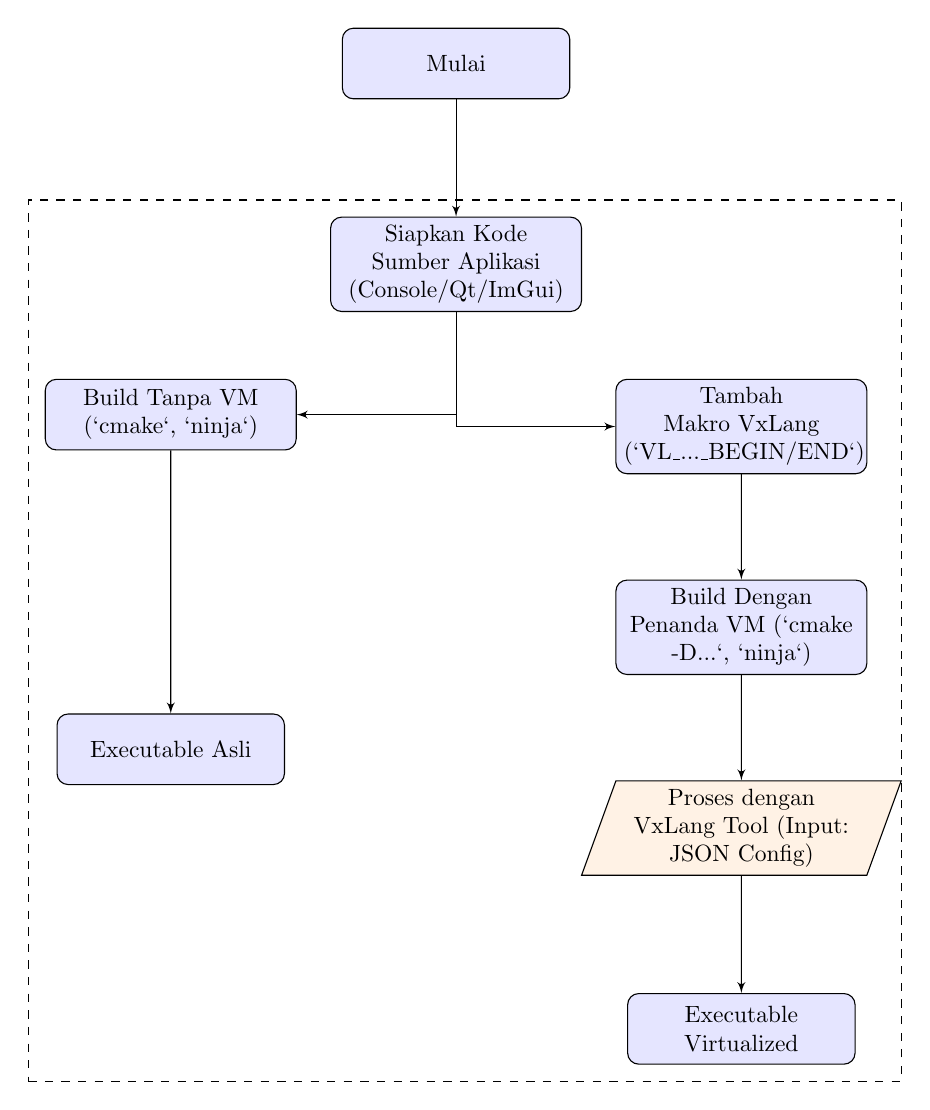
\begin{tikzpicture}[
        scale=0.85, transform shape, % Skala diagram & teks
        node distance=3cm and 2.2cm, % Jarak antar node
        >=latex,
        block/.style={rectangle, draw, fill=blue!10, text width=9em, text centered, rounded corners, minimum height=3em},
        line/.style={draw, -latex'},
        io/.style={trapezium, trapezium left angle=70, trapezium right angle=110, draw, fill=orange!10, text centered, minimum height=2em}
    ]
        % Nodes
        \node [block] (start) {Mulai};
        \node [block, below of=start, text width=10em] (prep_code) {Siapkan Kode Sumber Aplikasi (Console/Qt/ImGui)};
        \node [block, below left=1cm and 0.5cm of prep_code, text width=10em] (build_no_vm) {Build Tanpa VM (`cmake`, `ninja`)};
        \node [block, below right=1cm and 0.5cm of prep_code, text width=10em] (add_macro) {Tambah Makro VxLang (`VL\_...\_BEGIN/END`)};
        \node [block, below of=add_macro, text width=10em] (build_with_vm) {Build Dengan Penanda VM (`cmake -D...`, `ninja`)};
        \node [io, below of=build_with_vm, text width=10em] (vx_tool) {Proses dengan VxLang Tool (Input: JSON Config)};
        \node [block, below of=build_no_vm, yshift=-2cm] (exe_asli) {Executable Asli};
        \node [block, below of=vx_tool] (exe_vm) {Executable Virtualized};

        % Paths
        \path [line] (start) -- (prep_code);
        \path [line] (prep_code) |- (build_no_vm);
        \path [line] (prep_code) |- (add_macro);
        \path [line] (add_macro) -- (build_with_vm);
        \path [line] (build_with_vm) -- (vx_tool);
        \path [line] (build_no_vm) -- (exe_asli);
        \path [line] (vx_tool) -- (exe_vm);

        % Grouping Preparation
        \node [draw, dashed, inner sep=6pt, fit=(prep_code) (build_no_vm) (add_macro) (build_with_vm) (vx_tool) (exe_asli) (exe_vm)] {};
    \end{tikzpicture}
    \caption{Diagram Alur Persiapan Executable untuk Pengujian Autentikasi.}
    \label{fig:flow_auth_prep_rev} % Label SETELAH caption
\end{figure}
%--- AKHIR DIAGRAM PERSIAPAN AUTH ---

%--- DIAGRAM ANALISIS AUTH ---
\begin{figure}[htbp]
    \centering
    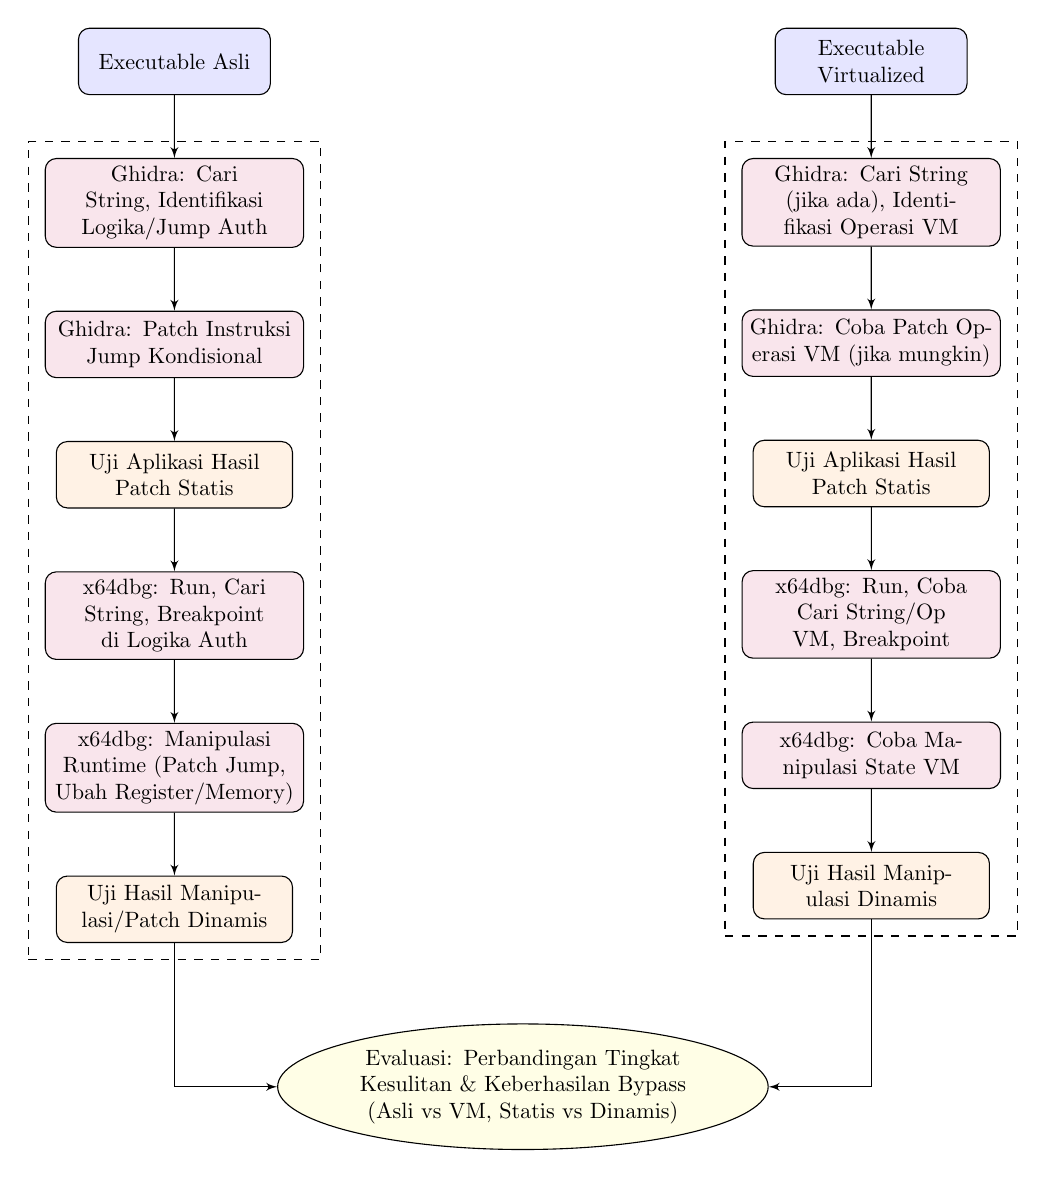
\begin{tikzpicture}[
        scale=0.8, transform shape,
        node distance=1.5cm and 1cm,
        >=latex,
        block/.style={rectangle, draw, fill=blue!10, text width=8em, text centered, rounded corners, minimum height=3em},
        proc/.style={rectangle, draw, fill=purple!10, text width=11em, text centered, rounded corners, minimum height=3em},
        test/.style={rectangle, draw, fill=orange!10, text width=10em, text centered, rounded corners, minimum height=3em},
        result/.style={ellipse, draw, fill=yellow!10, text centered, minimum height=3em, text width=15em},
        line/.style={draw, -latex'}
    ]
        % Input Executables
        \node [block] (exe_asli) {Executable Asli};
        \node [block, right=8cm of exe_asli] (exe_vm) {Executable Virtualized};

        % Static Analysis / Patching Path
        \node [proc, below=1cm of exe_asli] (static_ghidra_asli) {Ghidra: Cari String, Identifikasi Logika/Jump Auth};
        \node [proc, below=1cm of exe_vm] (static_ghidra_vm) {Ghidra: Cari String (jika ada), Identifikasi Operasi VM};
        \node [proc, below=1cm of static_ghidra_asli] (static_patch_asli) {Ghidra: Patch Instruksi Jump Kondisional};
        \node [proc, below=1cm of static_ghidra_vm] (static_patch_vm) {Ghidra: Coba Patch Operasi VM (jika mungkin)};
        \node [test, below=1cm of static_patch_asli] (static_test_asli) {Uji Aplikasi Hasil Patch Statis};
        \node [test, below=1cm of static_patch_vm] (static_test_vm) {Uji Aplikasi Hasil Patch Statis};

        % Dynamic Analysis / Manipulation Path
        \node [proc, below=1cm of static_test_asli] (dynamic_x64_asli) {x64dbg: Run, Cari String, Breakpoint di Logika Auth};
        \node [proc, below=1cm of static_test_vm] (dynamic_x64_vm) {x64dbg: Run, Coba Cari String/Op VM, Breakpoint};
        \node [proc, below=1cm of dynamic_x64_asli] (dynamic_manip_asli) {x64dbg: Manipulasi Runtime (Patch Jump, Ubah Register/Memory)};
        \node [proc, below=1cm of dynamic_x64_vm] (dynamic_manip_vm) {x64dbg: Coba Manipulasi State VM};
        \node [test, below=1cm of dynamic_manip_asli] (dynamic_test_asli) {Uji Hasil Manipulasi/Patch Dinamis};
        \node [test, below=1cm of dynamic_manip_vm] (dynamic_test_vm) {Uji Hasil Manipulasi Dinamis};

        % Evaluation
        \node [result, below=2cm of $(dynamic_test_asli)!0.5!(dynamic_test_vm)$] (eval_result) {Evaluasi: Perbandingan Tingkat Kesulitan \& Keberhasilan Bypass (Asli vs VM, Statis vs Dinamis)};

        % Paths
        % Static
        \path [line] (exe_asli) -- (static_ghidra_asli);
        \path [line] (exe_vm) -- (static_ghidra_vm);
        \path [line] (static_ghidra_asli) -- (static_patch_asli);
        \path [line] (static_ghidra_vm) -- (static_patch_vm);
        \path [line] (static_patch_asli) -- (static_test_asli);
        \path [line] (static_patch_vm) -- (static_test_vm);
        % Dynamic
        \path [line] (static_test_asli) -- (dynamic_x64_asli);
        \path [line] (static_test_vm) -- (dynamic_x64_vm);
        \path [line] (dynamic_x64_asli) -- (dynamic_manip_asli);
        \path [line] (dynamic_x64_vm) -- (dynamic_manip_vm);
        \path [line] (dynamic_manip_asli) -- (dynamic_test_asli);
        \path [line] (dynamic_manip_vm) -- (dynamic_test_vm);
        % Evaluation
        \path [line] (dynamic_test_asli) |- (eval_result);
        \path [line] (dynamic_test_vm) |- (eval_result);

        % Optional Grouping
         \node [draw, dashed, inner sep=6pt, fit=(static_ghidra_asli)(static_patch_asli)(static_test_asli)(dynamic_x64_asli)(dynamic_manip_asli)(dynamic_test_asli)] {};
        \node [draw, dashed, inner sep=6pt, fit=(static_ghidra_vm)(static_patch_vm)(static_test_vm)(dynamic_x64_vm)(dynamic_manip_vm)(dynamic_test_vm)] {};

    \end{tikzpicture}
    \caption{Diagram Alur Analisis Upaya Bypass Autentikasi.}
    \label{fig:flow_auth_analysis_rev} % Label SETELAH caption
\end{figure}
%--- AKHIR DIAGRAM ANALISIS AUTH ---

\subsection{Aplikasi Studi Kasus Autentikasi}
Tiga jenis aplikasi dengan dua varian mekanisme autentikasi dikembangkan:

\begin{enumerate}
    \item \bo{Aplikasi Konsol (\code{console}, \code{console\_cloud}):} Aplikasi CLI sederhana.
        \begin{itemize}
            \item \bo{Varian Hardcoded (\code{src/console/console.cpp}):} Membandingkan input \code{std::cin} dengan \f{string} literal (\f{"seno"}, \f{"rahman"}) menggunakan \code{std::string::compare()}.
            \item \bo{Varian Cloud (\code{src/console/console\_cloud.cpp}):} Menggunakan \code{send\_login\_request} dari \code{includes/cloud.hpp} untuk mengirim kredensial via HTTP POST ke \code{http://localhost:9090/login}.
        \end{itemize}
    \item \bo{Aplikasi Qt (\code{app\_qt}, \code{app\_qt\_cloud}):} Aplikasi GUI menggunakan Qt Widgets. UI dari \code{src/app\_qt/forms/todo\_auth.ui}.
        \begin{itemize}
            \item \bo{Varian Hardcoded (\code{src/app\_qt/src/todo\_auth.cpp}):} Logika perbandingan \f{hardcoded} dalam \f{slot} \code{on\_button\_login\_clicked()} menggunakan \code{QLineEdit::text()}. Menampilkan hasil via \code{QMessageBox}.
            \item \bo{Varian Cloud (\code{src/app\_qt/src/todo\_auth\_cloud.cpp}):} \f{Slot} memanggil \code{send\_login\_request} dan menampilkan \code{QMessageBox} berdasarkan respons.
        \end{itemize}
    \item \bo{Aplikasi Dear ImGui (\code{app\_imgui}, \code{app\_imgui\_cloud}):} Aplikasi GUI \f{immediate mode} menggunakan Dear ImGui, GLFW, OpenGL.
        \begin{itemize}
            \item \bo{Varian Hardcoded (\code{src/app\_imgui/login.cpp}):} Logika perbandingan dalam \code{Login::LoginWindow} saat \code{ImGui::Button("Login")} ditekan. Hasil ditampilkan via \code{MessageBoxW}.
            \item \bo{Varian Cloud (\code{src/app\_imgui/login\_cloud.cpp}):} Memanggil \code{send\_login\_request} saat tombol login ditekan, menampilkan hasil via \code{MessageBoxW}.
        \end{itemize}
\end{enumerate}

\subsection{Integrasi VxLang pada Aplikasi Autentikasi}
Integrasi VxLang dilakukan secara selektif pada logika autentikasi:

\begin{enumerate}
    \item \bo{Penyertaan Header:} \code{\#include "vxlang/vxlib.h"} ditambahkan pada file \code{.cpp} yang relevan.
    \item \bo{Penautan Library:} \code{vxlib64.lib} ditautkan ke target via \code{target\_link\_libraries} di \code{CMakeLists.txt}.
    \item \bo{Penempatan Makro Penanda:} \code{VL\_VIRTUALIZATION\_BEGIN} dan \code{VL\_VIRTUALIZATION\_END} membungkus blok kode autentikasi. Contoh pada \code{src/console/console.cpp}:
          \begin{minted}{cpp}
int main(int, char *[]) {
  // ... input username/password ...

  VL_VIRTUALIZATION_BEGIN; // <-- Makro awal

  if (inputUsername.compare("seno") == 0 &&
      inputPassword.compare("rahman") == 0) {
    std::cout << "Authorized!" << std::endl;
  } else {
    std::cout << "Not authorized." << std::endl;
  }

  VL_VIRTUALIZATION_END; // <-- Makro akhir

  system("pause");
  return 0;
}
          \end{minted}
          Pada varian \f{cloud}, makro membungkus pemanggilan \code{send\_login\_request} dan penanganan responsnya.
    \item \bo{Manajemen Build via CMake:} Opsi CMake \code{USE\_VL\_MACRO} mengontrol aktivasi makro.
        \begin{itemize}
            \item Jika aktif (\code{-DUSE\_VL\_MACRO=1}): Definisi \code{USE\_VL\_MACRO} ditambahkan, mengaktifkan fungsi makro di \code{vxlib.h}. Nama output diubah menjadi \code{*\_vm.exe}.
            \item Jika tidak aktif: Makro menjadi kosong. Nama output standar.
        \end{itemize}
\end{enumerate}

\subsection{Implementasi Sisi Server (Varian Cloud)}
\f{Backend} API lokal untuk varian \f{cloud} diimplementasikan sebagai berikut:

\begin{itemize}
    \item \bo{Teknologi:} Go (Golang) untuk API (\code{server/backend/main.go}), PostgreSQL 15 untuk database, Docker dan Docker Compose untuk \f{deployment} (\code{server/docker-compose.yml}).
    \item \bo{API Endpoint \code{/login} (POST):} Menerima JSON, mengambil \f{salt/hash} dari DB, menghitung ulang \f{hash} input menggunakan PBKDF2-SHA256 (100k iterasi), membandingkan \f{hash} (\f{constant time}), mengembalikan \code{{"success": true/false}}.
    \item \bo{API Endpoint \code{/register} (POST):} Menerima JSON, generate \f{salt}, hitung \f{hash} PBKDF2, simpan ke DB.
    \item \bo{Database Schema (\code{server/postgres/init.sql}):} Tabel \code{users(username, password\_hash, salt)}. Menyisipkan user \f{default} (\f{seno}/rahman) dengan \f{hash/salt} precomputed.
\end{itemize}

%-----------------------------------------------------------------------------%
\section{Implementasi Pengujian Performa}
%-----------------------------------------------------------------------------%
Pengujian ini mengukur dampak kuantitatif VxLang pada kecepatan eksekusi dan ukuran \f{executable}. Diagram alur untuk persiapan dan pelaksanaan pengujian performa disajikan pada Gambar \ref{fig:flow_perf_rev}.

%--- DIAGRAM PERF ---

\begin{figure}[htbp]
\centering
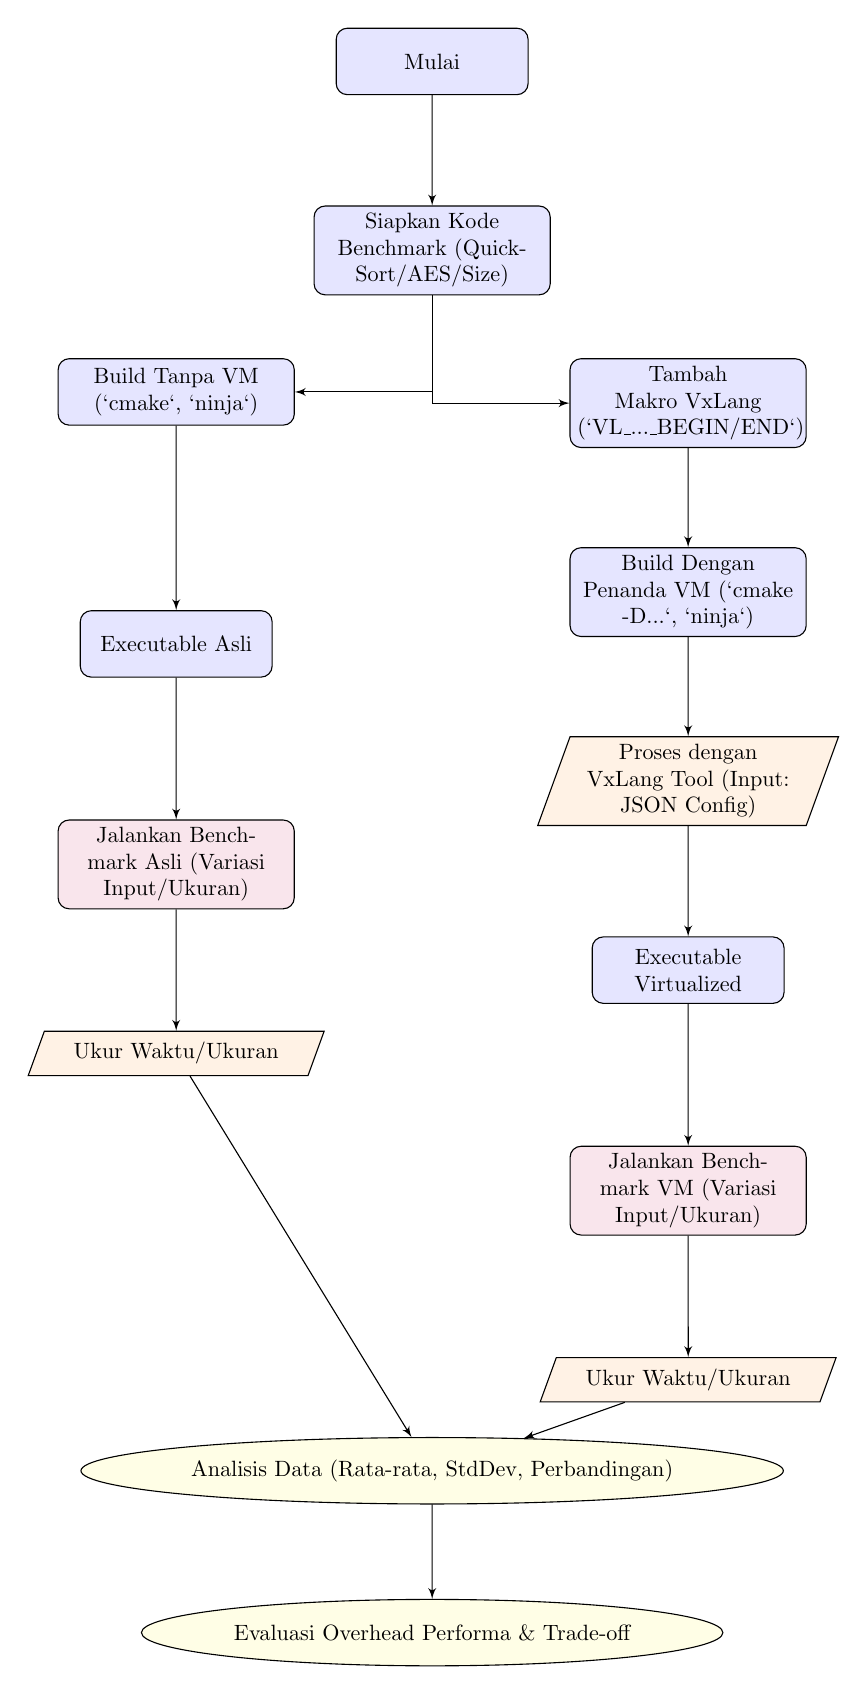
\begin{tikzpicture}[
scale=0.8, transform shape, % <<-- Skala lebih kecil
node distance=3cm and 1.5cm, % <<-- Kurangi jarak horizontal
>=latex,
block/.style={rectangle, draw, fill=blue!10, text width=8em, text centered, rounded corners, minimum height=3em},
proc/.style={rectangle, draw, fill=purple!10, text width=10em, text centered, rounded corners, minimum height=3em},
result/.style={ellipse, draw, fill=yellow!10, text centered, minimum height=3em},
io/.style={trapezium, trapezium left angle=70, trapezium right angle=110, draw, fill=orange!10, text centered, minimum height=2em},
line/.style={draw, -latex'}
]
  % Nodes
  \node [block] (start) {Mulai};
  \node [block, below of=start, text width=10em] (prep_code) {Siapkan Kode Benchmark (QuickSort/AES/Size)};
    % Kolom Kiri (Asli)
    \node [block, below left=1cm and 0.3cm of prep_code, text width=10em] (build_no_vm) {Build Tanpa VM (`cmake`, `ninja`)}; % Geser lebih dekat
    \node [block, below of=build_no_vm, yshift=-1cm] (exe_asli) {Executable Asli}; % Sesuaikan posisi vertikal jika perlu
    \node [proc, below of=exe_asli, yshift=-0.5cm] (run_bench_asli) {Jalankan Benchmark Asli (Variasi Input/Ukuran)};
    \node [io, below of=run_bench_asli] (measure_asli) {Ukur Waktu/Ukuran};

    % Kolom Kanan (VM)
    \node [block, below right=1cm and 0.3cm of prep_code, text width=10em] (add_macro) {Tambah Makro VxLang (`VL\_...\_BEGIN/END`)}; % Geser lebih dekat
    \node [block, below of=add_macro, text width=10em] (build_with_vm) {Build Dengan Penanda VM (`cmake -D...`, `ninja`)};
    \node [io, below of=build_with_vm, text width=10em] (vx_tool) {Proses dengan VxLang Tool (Input: JSON Config)};
    \node [block, below of=vx_tool] (exe_vm) {Executable Virtualized};
    \node [proc, below of=exe_vm, yshift=-0.5cm] (run_bench_vm) {Jalankan Benchmark VM (Variasi Input/Ukuran)};
    \node [io, below of=run_bench_vm] (measure_vm) {Ukur Waktu/Ukuran};

    % Nodes Tengah Bawah
    \node [result, below=3.5cm of $(measure_asli)!0.5!(measure_vm)$] (analyze_data) {Analisis Data (Rata-rata, StdDev, Perbandingan)}; % Geser ke tengah
    \node [result, below=1.5cm of analyze_data] (eval_overhead) {Evaluasi Overhead Performa \& Trade-off};

    % Paths
    \path [line] (start) -- (prep_code);
    \path [line] (prep_code) |- (build_no_vm);
    \path [line] (prep_code) |- (add_macro);
    \path [line] (add_macro) -- (build_with_vm);
    \path [line] (build_with_vm) -- (vx_tool);
    \path [line] (build_no_vm) -- (exe_asli);
    \path [line] (vx_tool) -- (exe_vm);

    \path [line] (exe_asli) -- (run_bench_asli);
    \path [line] (exe_vm) -- (run_bench_vm);
    \path [line] (run_bench_asli) -- (measure_asli);
    \path [line] (run_bench_vm) -- (measure_vm);
    \path [line] (measure_asli) -- (analyze_data);
    \path [line] (measure_vm) -- (analyze_data);
    \path [line] (analyze_data) -- (eval_overhead);

    % Grouping (Optional) - Mungkin hapus jika terlalu lebar
    % \node [draw, dashed, inner sep=6pt, fit=(prep_code) (build_no_vm) (add_macro) (build_with_vm) (vx_tool) (exe_asli) (exe_vm)] {};
    % \node [draw, dashed, inner sep=6pt, fit=(run_bench_asli) (run_bench_vm) (measure_asli) (measure_vm) (analyze_data) (eval_overhead)] {};
\end{tikzpicture}
\caption{Diagram Alur Persiapan dan Pengujian Performa.}
\label{fig:flow_perf_rev} % Label SETELAH caption
\end{figure}

%--- AKHIR DIAGRAM PERF ---

\subsection{Benchmark Algoritma Quick Sort (\code{QuickSort})}
\begin{itemize}
    \item \bo{Implementasi (\code{src/performance/quick\_sort.cpp}):} Menggunakan \code{std::vector<int>}, fungsi rekursif \code{quickSort}, dan \code{partition}.
    \item \bo{Data:} Vektor acak (1-1.000.000) ukuran bervariasi (100 s/d 3.000.000 elemen).
    \item \bo{Pengukuran:} \code{std::chrono::high\_resolution\_clock} mengukur waktu eksekusi \code{quickSort}. Diulang 100 kali per ukuran data. Rata-rata dan standar deviasi dihitung.
    \item \bo{Integrasi VxLang:} \code{VL\_VIRTUALIZATION\_BEGIN/END} membungkus \textit{seluruh isi} fungsi rekursif \code{quickSort}.
\end{itemize}

\subsection{Benchmark Enkripsi AES-CBC-256 (\code{Encryption})}
\begin{itemize}
    \item \bo{Implementasi:} Kelas \code{AESCipher} (\code{aes.h}, \code{aes.cpp}) menggunakan API \code{EVP} OpenSSL untuk AES-256-CBC.
    \item \bo{Data:} 1 GB data acak (1 juta blok @ 1024 byte), diproses per \f{batch} (misal, 10.000 blok/batch).
    \item \bo{Pengukuran:} \code{chrono} mengukur total waktu enkripsi/dekripsi seluruh \f{batch}. \f{Throughput} (MB/s) dihitung.
    \item \bo{Integrasi VxLang:} \code{VL\_VIRTUALIZATION\_BEGIN/END} membungkus \f{looping} pemanggilan \code{aes.encrypt()}/\code{decrypt()} di dalam fungsi \code{measureBatch...Time}.
\end{itemize}

\subsection{Pengukuran Ukuran File}
\begin{itemize}
    \item \bo{Implementasi:} Ukuran file \f{executable} diukur menggunakan fungsi \code{std::filesystem::file\_size} atau melalui \f{file explorer} Windows. Aplikasi \code{Size} (\code{src/performance/size.cpp}) dibuat khusus dengan data \textit{dummy} tersemat (\code{dummy.bin} via \code{dummy.rc}) untuk mensimulasikan aplikasi dengan aset data internal yang besar.
    \item \bo{Target Pengukuran:} Pengukuran ukuran file dilakukan pada \textbf{semua} target \f{executable} yang dihasilkan, baik versi asli maupun versi \textit{virtualized} (\code{*\_vm.exe}), termasuk \code{QuickSort}, \code{Encryption}, \code{Size}, \code{console}, \code{app\_imgui}, dan \code{app\_qt}, sesuai data pada Tabel \ref{tab:file_size}.
    \item \bo{Integrasi VxLang pada Target \code{Size}:} Makro \code{VL\_VIRTUALIZATION\_BEGIN/END} tetap disertakan dalam \code{main} pada target \code{Size} untuk memastikan \f{runtime} VxLang disertakan pada versi \code{size\_vm.exe}, sehingga memungkinkan perbandingan ukuran yang fokus pada \textit{overhead} \textit{runtime} itu sendiri.
\end{itemize}

%-----------------------------------------------------------------------------%
\section{Proses Kompilasi dan Virtualisasi}
%-----------------------------------------------------------------------------%
Alur kerja untuk menghasilkan \f{executable} asli dan yang tervirtualisasi adalah:

\begin{enumerate}
    \item \bo{Konfigurasi CMake:} Menjalankan \code{cmake -G Ninja -B build [-DUSE\_VL\_MACRO=1] ..}. Opsi \code{-DUSE\_VL\_MACRO=1} ditambahkan jika membangun untuk virtualisasi.
    \item \bo{Kompilasi Awal:} Menjalankan \code{ninja -C build}. Menghasilkan \code{*.exe} (jika \code{USE\_VL\_MACRO} nonaktif) atau \code{*\_vm.exe} (jika \code{USE\_VL\_MACRO} aktif, berisi penanda).
    \item \bo{Proses Virtualisasi Eksternal:} \f{Executable} \code{*\_vm.exe} dari langkah 2 diproses oleh \textbf{tool eksternal VxLang} (tidak ada dalam repositori ini). Tool ini, dikonfigurasi via file JSON, membaca penanda, menerjemahkan kode menjadi \f{bytecode}, dan menyematkan \f{interpreter} VM ke \f{executable} output.
    \item \bo{Hasil Akhir:} Direktori \code{bin} berisi \f{executable} asli (\code{*.exe}) dan \f{executable} yang telah divirtualisasi (\code{*\_vm.exe}), siap untuk dianalisis.
\end{enumerate}

Implementasi yang sistematis ini memastikan bahwa artefak yang dihasilkan cocok untuk perbandingan dan analisis yang valid sesuai dengan tujuan penelitian.

%-----------------------------------------------------------------------------%
\chapter{\babLima}
%-----------------------------------------------------------------------------%

%-----------------------------------------------------------------------------%
\section{Saran}
%-----------------------------------------------------------------------------%


%-----------------------------------------------------------------------------%
\chapter{\babEnam}
%-----------------------------------------------------------------------------%

\section{Kesimpulan}

\section{Saran}


%\input{src/01-body/99-kesimpulan}

%
% Daftar Pustaka
% \input{pustaka.bib}

% Alternatif manajemen daftar pustaka dengan \bibliography
% \bibliographystyle{unsrt}
% \bibliography{pustaka}

% Custom manajemen daftar pustaka dengan \biblatex
\newpage
\phantomsection
\printbibliography[heading=bibintoc,title={\uppercase{Daftar Referensi}}]


\newcounter{lastMainPage} % Buat counter untuk menyimpan nomor halaman terakhir
\setcounter{lastMainPage}{\value{page}} % Simpan nomor halaman terakhir dari Daftar Referensi

\appendix % This is a command to switch to appendix mode

\clearpage % Pastikan kita memulai di halaman baru setelah halaman pembatas
\pagenumbering{arabic} % Setel ulang penomoran ke angka Arab (ini akan mereset halaman ke 1)
\setcounter{page}{\value{lastMainPage}} % Setel counter halaman ke nomor halaman terakhir Daftar Referensi
\addtocounter{page}{1} % Tambah 1, sehingga halaman pertama konten lampiran
                       % akan melanjutkan dari Daftar Referensi.

%
% @author  Andreas Febrian
% @version 1.00 
% 
% Hanya sebuah pembatas bertuliskan LAMPIRAN ditengah halaman. 
% 

\begin{titlepage}
	\centering 
	\vspace*{6cm}
	\noindent \Huge{LAMPIRAN}
	\addChapter{LAMPIRAN}
\end{titlepage} 


%-----------------------------------------------------------------------------%
%\addChapter{Lampiran 1}
%\chapter*{Lampiran 1}
%-----------------------------------------------------------------------------%


\end{document}
